\documentclass[11pt,a4paper]{article}

\usepackage[margin=1in]{geometry}
\usepackage[T1]{fontenc}
\usepackage{lmodern}
\usepackage{microtype}
\usepackage{amsmath,amssymb,amsthm}
\usepackage{graphicx}
\usepackage{booktabs}
\usepackage{enumitem}
\usepackage{subcaption}
\usepackage[dvipsnames]{xcolor}
\usepackage[numbers,sort&compress]{natbib}
\usepackage[colorlinks=true,linkcolor=blue!50!black,citecolor=blue!50!black,urlcolor=blue!50!black]{hyperref}
\usepackage[capitalise,noabbrev]{cleveref}
\usepackage{xurl}
\usepackage{orcidlink}

\graphicspath{{../figures/}}

\newtheorem{lemma}{Lemma}
\newtheorem{proposition}{Proposition}
\newtheorem{observation}{Observation}
\theoremstyle{remark}
\newtheorem{remark}{Remark}

\newcommand{\R}{\mathbb{R}}
\newcommand{\C}{\mathbb{C}}
\newcommand{\Sph}{\mathbb{S}}
\newcommand{\code}[1]{\texttt{#1}}
\newcommand{\smin}{\operatorname{smin}}
\newcommand{\Lk}{\operatorname{Lk}}
\DeclareMathOperator{\atan}{atan2}

\title{From Horned Spheres to Hopf Trees: Linking Graphs, M\"obius Invariants, and Coxeter Reflection Families}
\author{Brent Hartshorn \orcidlink{0009-0004-2853-655X}}

\begin{document}
\maketitle

\begin{abstract}
We model Alexander's horned sphere as an exact recursive distance field, whose
pruned breadth-first search we prove equal to the full minimum over all rings.  
Treating the horned sphere's ring tree and the Hopf fibres as two families of circles, 
we compute Gauss linking numbers over whole networks.  
Hopf fibres form a complete linking graph; the horned tree links only sibling pairs.  
A horned-style tree whose clasped pairs are Hopf pairs has the same sibling-only graph for most placements, 
but in a window of placements with thick, 
non-overlapping tubes every ring that has grandchildren is also linked to two of them, with signs $-1$ and $+1$, at depths 3 and 4.  

Finally, using the M\"obius invariants of circle pairs, we show that the horned sphere's clasp has invariants $(|1-2(\kappa-1)^2|,0)$, a Hopf pair exactly at $\kappa=1+1/\sqrt2$ and the oloid's pair at $\kappa=3/2$, 
that the Hopf tree at $\psi=180^\circ$ is the horned sphere at that clasp, and that the exact Hopf clasp is not distinguished by the number of links.  The Hopf and oloid clasps are members of a family $\kappa_n=1+\cos(\pi/2n)$ for which the ring and its children generate planar reflection groups with Coxeter relations; their limit sets are round circles.
\end{abstract}

\section{Introduction}

\begin{footnotesize}
\begin{equation}
\underbrace{s_1(\kappa)}_{\substack{\text{M\"obius clasp}\\\text{invariant (Sec.~9)}}}
= \overbrace{\bigl|\cos \theta_{cc}\bigr|}^{\substack{\text{child sphere}\\\text{angle (Sec.~10)}}}
= \underbrace{\bigl|1 - 2(\kappa - 1)^2\bigr|}_{\substack{\text{horned-sphere gap}\\\sin g = \kappa s \text{ (Sec.~6)}}}
= \begin{cases}
  0, & \kappa = 1 + \frac{1}{\sqrt{2}} \quad \text{(Hopf pair / }\psi = 180^\circ\text{ Hopf tree)}, \\[6pt]
  \frac{1}{2}, & \kappa = \frac{3}{2} \text{ or } 1 + \frac{\sqrt{3}}{2} \quad \text{(oloid two-circle roller)}, \\[6pt]
  \cos\!\left(\frac{\pi}{n}\right), & \kappa_n = 1 + \cos\!\left(\frac{\pi}{2n}\right) \quad \underbrace{\text{(Coxeter reflection group)}}_{s_m = \frac{\cos(\pi/m)}{\kappa_n}}.
\end{cases}
\end{equation}
\end{footnotesize}

\code{fractalkit}, written for exploration: 
where every fractal is a \emph{field}, a function from points of $\R^3$ to a distance estimate and an
orbit-trap value, and fields compose.  The aim is to be able to mix fractals, slice them, measure them and
combine them with other geometry, such as fibre networks and the Hopf fibration, in a few lines of Python.
This turned up structure that we found worth writing down:

\begin{enumerate}[leftmargin=*,itemsep=2pt]
\item The Hopfbrot's power map preserves the Hopf fibration, and induces on the base 2-sphere the angle-multiplying
  map of the 3D Mandelbulb (\cref{sec:hopfbrot}).  This gives a clean way to carry the 4D orbit through a 3D
  iteration framework.
\item The horned sphere admits an exact, order-independent distance estimate over a tree of rings, and a pruned
  breadth-first search that computes it exactly (\cref{sec:horned}).
\item The ring tree of the horned sphere and the fibres of the Hopf fibration are both families of linked circles;
  represented the same way, their linking graphs can be compared (\cref{sec:linking}).
\item If the clasped pair in each recursion step is a Hopf pair, the linking graph depends on one placement
  parameter.  In a window of that parameter the tubes can be thick and the graph is richer than the horned
  sphere's, and it follows a simple rule that repeats generation by generation (\cref{sec:hopftree}).
\item The clasp of the horned sphere has a closed-form M\"obius invariant; the exact Hopf clasp is one value of its \code{clasp} parameter, shared with the two-circle roller of a companion study of the Hopf fibration, and a Hopf tree is a horned sphere at that value (\cref{sec:clasp}).
\end{enumerate}

We also document two numerical pitfalls met on the way: a Gauss-integral artifact for touching curves, and
the bias of box-counting estimates (\cref{sec:numerics}).  Everything is reproducible from the repository and covered
by 69 automated tests (\cref{sec:repro}).  We state limitations, including what we did not prove, in
\cref{sec:limits}.

\section{Background and related work}

\paragraph{Distance estimation.}
John Hart (1989), Sandin and Kauffman introduced distance-estimated ray tracing of 3D deterministic fractals for quaternion Julia sets,
and Hart's sphere tracing (1996)~\cite{hart1996} marches a ray in steps given by a function that bounds the distance to the surface.
Dang, Kauffman and Sandin treat distance estimation for hypercomplex iterations rigorously~\cite{dang2002}.  For a map $z\mapsto f(z)+c$
the running-derivative estimate is $d \approx \tfrac12 |z|\ln|z| / |dz|$, the same form as the classical estimate
for the Mandelbrot set~\cite{peitgen1986}.  For the Mandelbulb it is a heuristic rather than a bound: Hvidtfeldt Christensen
discusses several approximations~\cite{hvidtfeldt_de}, and Quilez gives a widely used one~\cite{quilez_mandelbulb,quilez_distance}.

\paragraph{Bulbs and the Hopfbrot.}
The Mandelbulb arose on Fractal Forums in 2007--2009 from Daniel White's proposal to double the angles of a point in spherical coordinates, and
Paul Nylander's choice of a higher power~\cite{white2009}.  Knill's survey~\cite{knill2023} defines the degree-$d$ Hopfbrot, a name he
credits to Nylander, by the same angle-multiplying power map on the 3-sphere in Hopf coordinates.

\paragraph{The Hopf fibration.}
Hopf's map $h\colon \Sph^3\to\Sph^2$~\cite{hopf1931} has circles as fibres, and any two fibres are linked once; Lyons gives an elementary account
including the stereographic picture used here~\cite{lyons2003}.

\paragraph{The horned sphere.}
Alexander's 1924 construction~\cite{alexander1924} gives a 2-sphere embedded in $\R^3$ whose inside is simply connected but whose outside is not.
It has been modelled a few levels deep, for example as 3D-printed models~\cite{grillet2022}.

\paragraph{Linking numbers.}
The linking number of two disjoint oriented closed curves is the Gauss double integral, with equivalent definitions by degree and signed crossings~\cite{ricca2011,rolfsen1976}.
For polygons the integral can be computed exactly segment by segment~\cite{klenin2000}; here we use the simpler midpoint rule with local refinement (\cref{sec:linking}).


\section{A modular model}
\label{sec:model}

\paragraph{Fields.}
A \code{Field} has one method, \code{de(P)}, taking points $P$ of shape $(\dots,3)$ and returning a pair $(d,\tau)$:
a distance estimate $d$ (negative inside, for fields that have an inside) and an orbit-trap value $\tau\in[0,1]$ used for colouring.

Boolean and smooth operators act on fields:
union $\min$, intersection $\max$, subtraction $\max(a,-b)$, the quadratic smooth minimum
\begin{equation}
\smin(a,b;k)=\min(a,b)-\tfrac{k}{4}\,h^2,\qquad h=\frac{\max(k-|a-b|,0)}{k},
\label{eq:smin}
\end{equation}
a linear \emph{blend} $(1-t)\,d_A+t\,d_B$ (a morph, not a boolean), and the transforms \code{scaled}, \code{rotated}, \code{translated},
\code{repeated}, \code{warped} and \code{shell}.  Fields can also be built from a dictionary or JSON specification.

\paragraph{Iterated maps and hybrids.}
An \code{IterMap} splits an escape-time iteration into \code{start}, \code{step} and \code{finish}, acting on a vectorised state
$(c,z,\partial,\tau,\text{active},\text{extra})$: the sample point $c$, the orbit point $z\in\R^3$, a running derivative $\partial$, the trap, an
activity mask and a dictionary of per-map scratch.  A \code{Hybrid} interleaves the steps of several such maps according to a repeating
schedule, for instance two Hopfbrot steps then one Mandelbulb step, and finishes the distance with one chosen map.  The fold steps
(box fold, sphere fold, scaling, absolute value, rotation, offset) are \code{IterMap} steps too, which is how a Mandelbox or a kaleidoscopic IFS
is mixed with a bulb.  Hybrids are parameter-sensitive: the derivatives of different maps disagree, so expect speckle and use small step sizes
(\cref{fig:gallery}).

\begin{figure}[t]
\centering
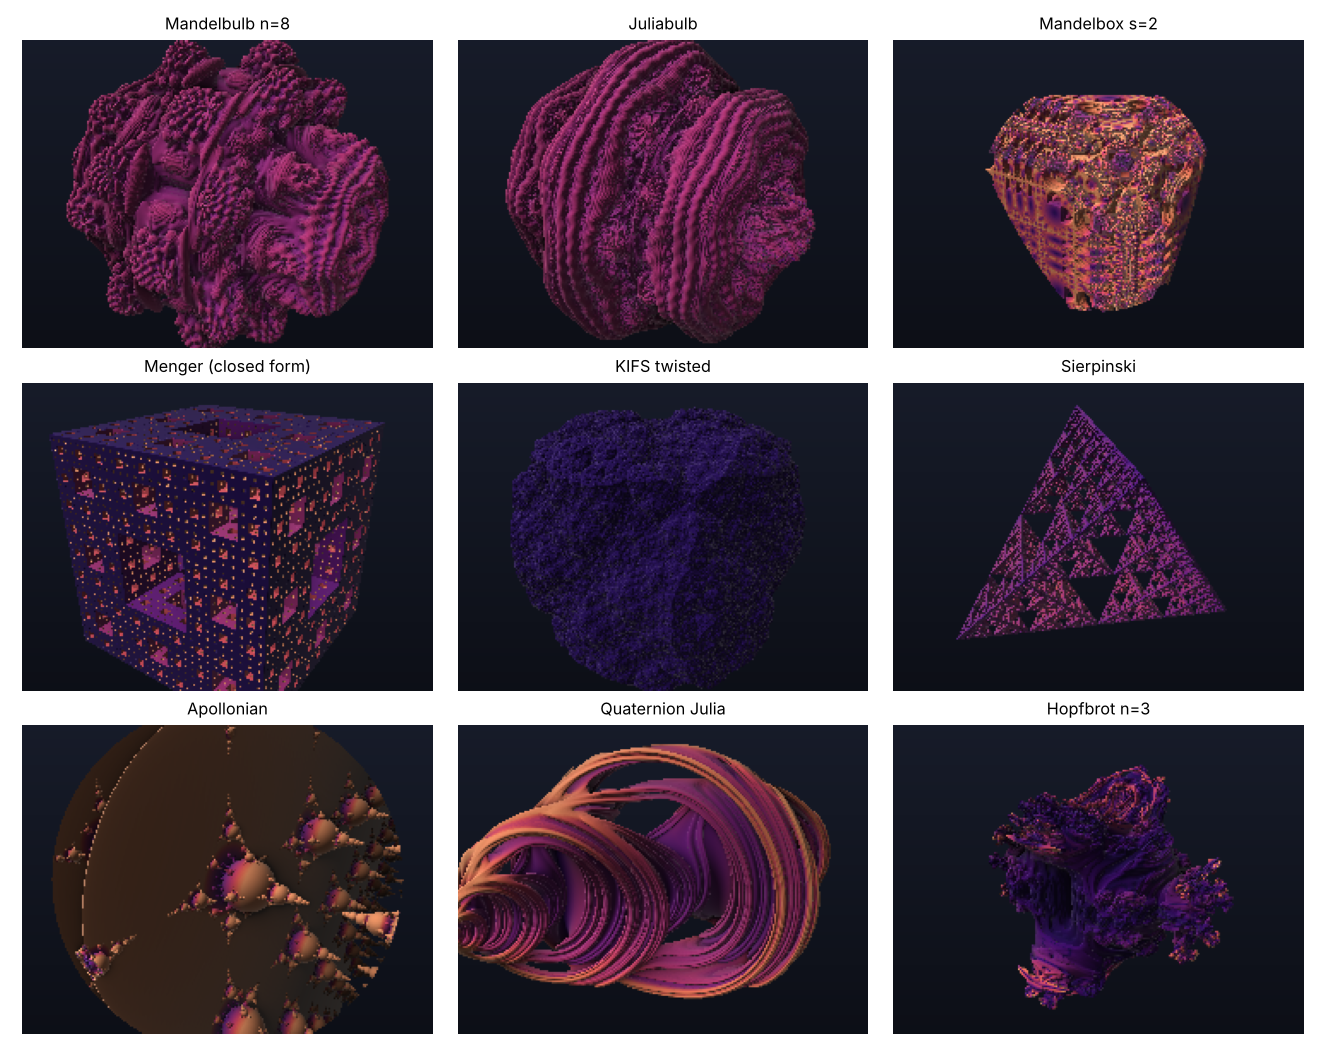
\includegraphics[width=0.78\linewidth]{gallery.png}\\[4pt]
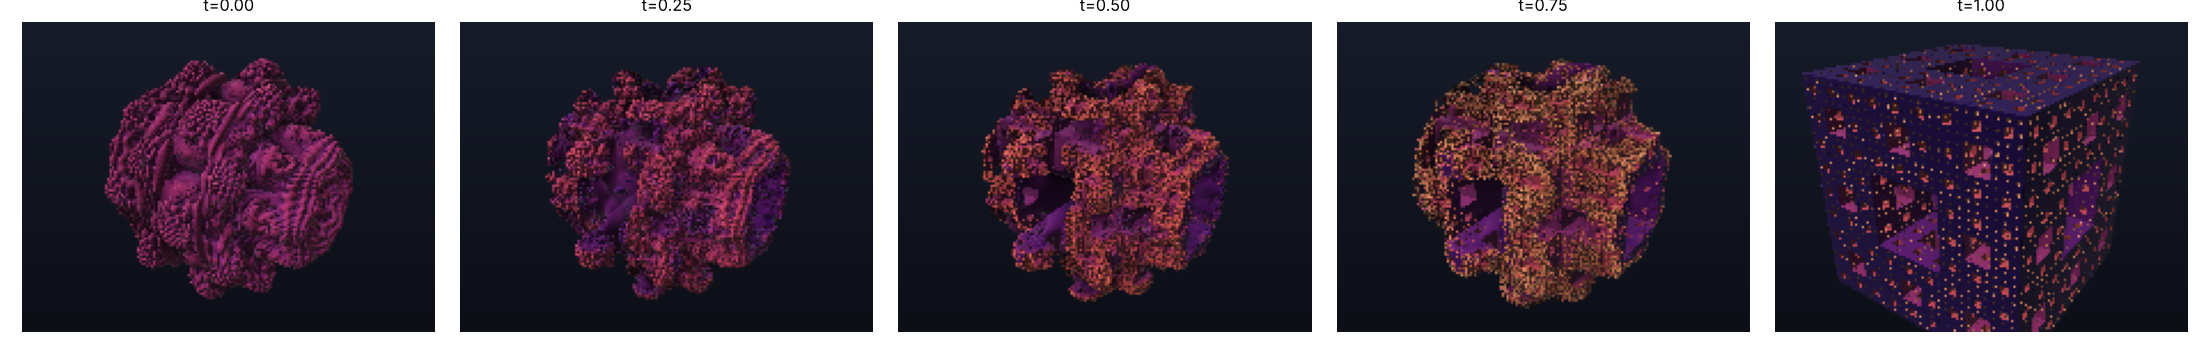
\includegraphics[width=\linewidth]{mix_morph.png}
\caption{Top: nine samples rendered by the numpy sphere tracer.  Bottom: a morph from a Mandelbulb ($t=0$) to a Menger sponge ($t=1$) by
linear blend of the two distance estimates, $t=0,\dots,1$ in steps of $0.25$.}
\label{fig:gallery}
\end{figure}

\begin{figure}[t]
\centering
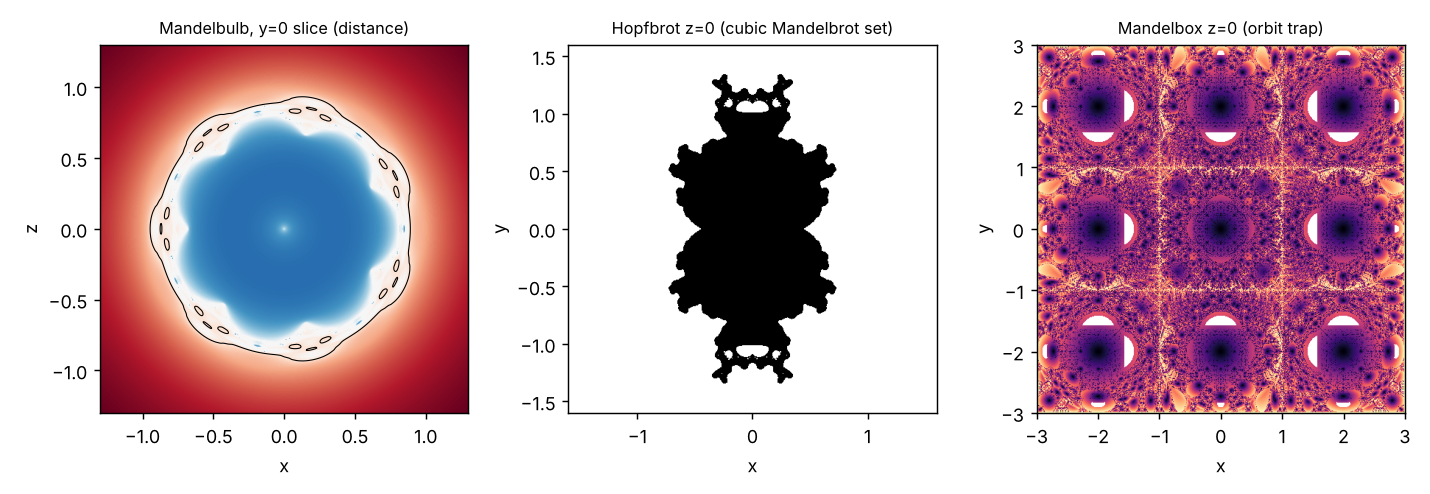
\includegraphics[width=\linewidth]{slices.png}
\caption{Slices evaluate \code{de} on a grid.  Left: a Mandelbulb distance field at $y=0$, with the surface contour.  Middle: the Hopfbrot of power 3 at $z=0$,
which is the cubic Mandelbrot set (\cref{sec:hopfbrot}).  Right: an orbit-trap slice of a Mandelbox.}
\label{fig:slices}
\end{figure}

\section{The Hopfbrot as an iterated map}
\label{sec:hopfbrot}

Write points of $\R^4\cong\C^2$ as $v=rU(\theta_1,\theta_2,\varphi)$ with $r=|v|$ and the Hopf parametrisation of $\Sph^3$,
\begin{equation}
U(\theta_1,\theta_2,\varphi)=(\cos\varphi\, e^{i\theta_1},\ \sin\varphi\, e^{i\theta_2}),\qquad \varphi\in[0,\tfrac{\pi}{2}].
\end{equation}
The degree-$n$ power map is $v^{\langle n\rangle}=r^{n}\,U(n\theta_1,n\theta_2,n\varphi)$, and the Hopfbrot iterates $w\mapsto w^{\langle n\rangle}+c$
from $w=c\in\R^4$~\cite{knill2023}.  ray samples $c$ from a 3D slice of $\R^4$:
$c=(x+\delta,\ y,\ z\cos\tau-\sigma\sin\tau,\ z\sin\tau+\sigma\cos\tau)$ with tilt $\tau$, offset $\sigma$, and a shift $\delta=-\tfrac12\max(3-n,0)$ that centres the degree 2 set.
The distance estimate is $d=\tfrac12\,|w|\ln|w|/\partial$ with $\partial\leftarrow n|w|^{n-1}\partial+1$.

\paragraph{The power map respects the fibration.}
Let $h(z_1,z_2)=(|z_1|^2-|z_2|^2,\ 2z_1\bar z_2)\in\R\times\C\cong\R^3$ be the Hopf map, whose fibres are the circles $(e^{it}z_1,e^{it}z_2)$.

\begin{proposition}\label{prop:hopf}
For $\varphi\in[0,\pi/2]$ and $\alpha=\theta_1-\theta_2$,
\begin{equation}
h\bigl(U(\theta_1,\theta_2,\varphi)\bigr)=\bigl(\cos2\varphi,\ \sin2\varphi\,e^{i\alpha}\bigr),
\end{equation}
so $h\circ(\,\cdot\,)^{\langle n\rangle}=B_n\circ h$ on $\Sph^3$ with
\begin{equation}
B_n(\cos\vartheta,\ \sin\vartheta\,e^{i\alpha})=(\cos n\vartheta,\ \sin n\vartheta\,e^{in\alpha}).
\end{equation}
In particular the angular part of the power map sends every fibre into a fibre, and the induced map on the base sphere $\Sph^2$ is the
map that multiplies the polar angle $\vartheta=2\varphi$ and the azimuth $\alpha$ by $n$: the angular map of the $n$-th power Mandelbulb.
\end{proposition}
\begin{proof}
$2z_1\bar z_2=2\cos\varphi\sin\varphi\,e^{i(\theta_1-\theta_2)}$ and $|z_1|^2-|z_2|^2=\cos2\varphi$.  The power map replaces $(\theta_1,\theta_2,\varphi)$
by $(n\theta_1,n\theta_2,n\varphi)$, which replaces $(\vartheta,\alpha)=(2\varphi,\theta_1-\theta_2)$ by $(n\vartheta,n\alpha)$.  A fibre is a curve along which
$\varphi$ and $\alpha$ are constant, so its image has $n\varphi$ and $n\alpha$ constant.
\end{proof}

We checked the identity numerically on $2000$ random points to $10^{-14}$.  Two remarks.  First, the proposition concerns only the angular part:
the radius is free, and the added $c$ destroys fibre preservation after the first step, so it is a statement about the map and not about the
orbits.  Second, if $c$ has vanishing last two coordinates then $\varphi=0$ is invariant and the iteration is the complex map $w\mapsto w^n+c$ on the
plane $\{w_3=w_4=0\}$.  That is why the $z=0$ plane of the default slice holds the Mandelbrot set of degree $n$, the codimension-two trace
described by Knill~\cite{knill2023}; we confirm that the orbit of our implementation equals the complex orbit to $3\times10^{-15}$ for $n=3$ (\cref{fig:slices}, middle).

\paragraph{Carrying a 4D orbit in a 3D framework.}
The \code{IterMap} state keeps $z\in\R^3$.  The Hopfbrot stores the first three coordinates of $w$ in $z$ and the fourth in the scratch
entry \code{extra["w4"]}; the escape test and the distance estimate use the 4D norm.  Run alone, the map reproduces the original standalone kernel to
$10^{-12}$ on five parameter sets (powers 2, 3, 5; several tilts and offsets), including the four extra iterations ray runs for orbits still beyond radius 2.

Inside a \code{Hybrid} the semantics need stating, because a fold or bulb step knows nothing of the fourth coordinate.  The other maps act on $(w_1,w_2,w_3)$ and leave $w_4$
unchanged, which is the identity lift to 4D.  If the Hopfbrot is not the finishing map, its first step initialises $w_4$ from the sample point's fourth
slice coordinate, and the $+c$ it adds is the 4D slice point, not the raw sample.  The extra iterations are dropped.  Mixing it with a Mandelbulb, Mandelbox,
kaleidoscopic IFS or the Riemann sphere gives the shapes in \cref{fig:hopfbrot_hybrid}; we regard them as explorations, not as validated renderings: the estimates of different maps disagree and the
images are speckled.

\begin{figure}[t]
\centering
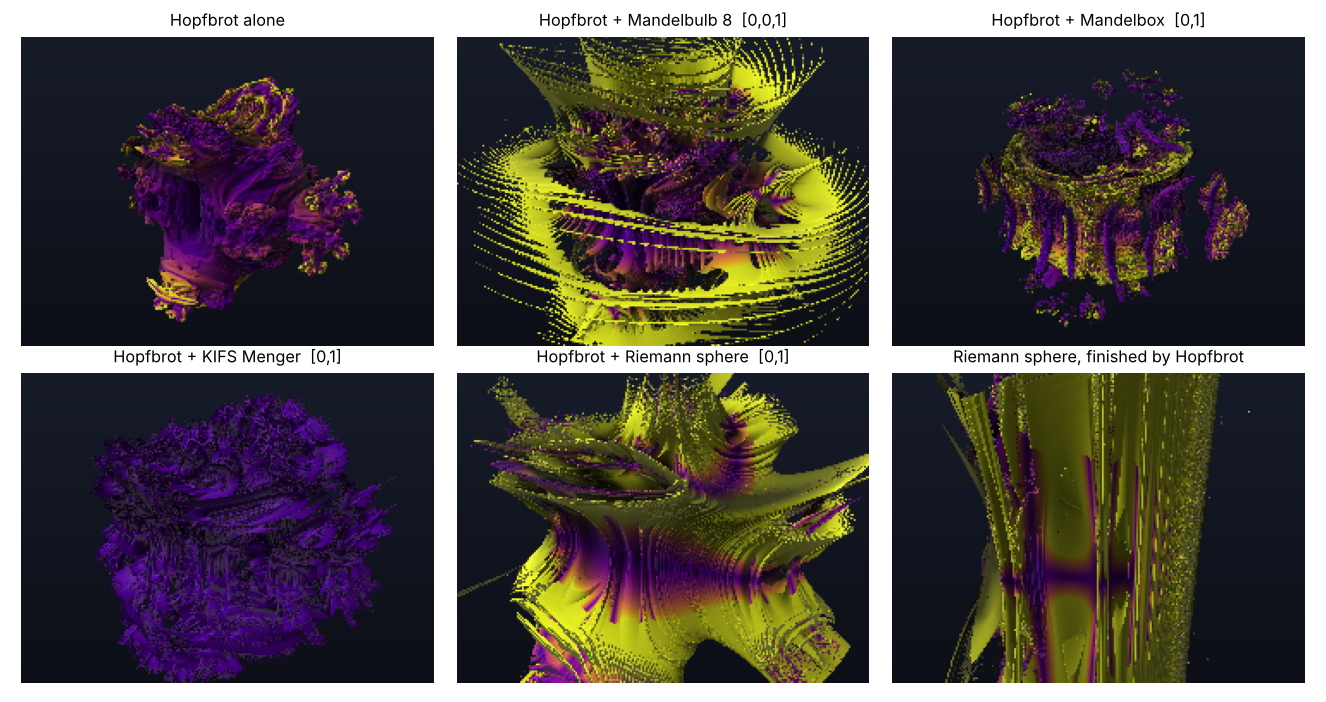
\includegraphics[width=0.8\linewidth]{hopfbrot_hybrid.png}\\[6pt]
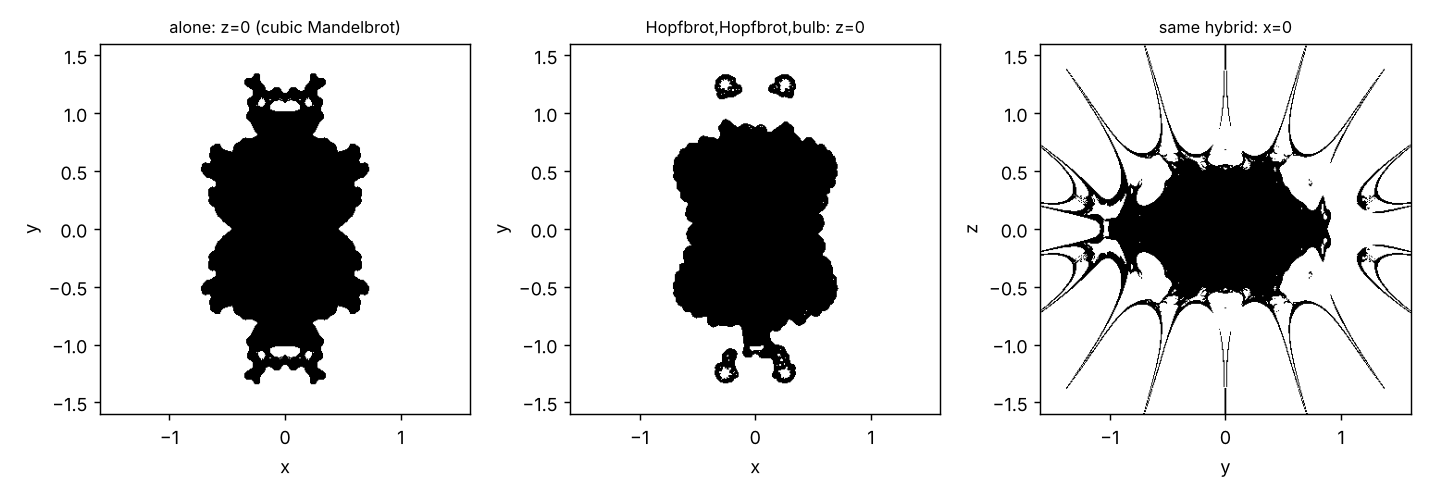
\includegraphics[width=0.95\linewidth]{hopfbrot_slices.png}
\caption{Top: the Hopfbrot alone and in five hybrids (schedules in brackets: $[0,0,1]$ is two steps of the first map then one of the second).  Bottom: slices at $z=0$ of the
Hopfbrot alone and of the Hopfbrot--Mandelbulb hybrid, and at $x=0$ of the hybrid.}
\label{fig:hopfbrot_hybrid}
\end{figure}

\section{The Riemann-sphere map}
\label{sec:riemann}

The Riemann-sphere fractal folds the plane after a stereographic projection.  With $R$ the \code{radius} parameter, offsets $(a_1,a_2)$, a constant $c_0$ (default $(0,1,0)$) and a weight $\mu$ on the sample
point $P$ (\code{mandel}), one step from $z$ with $r=|z|$ is as follows.  Put $u=Rz/r$ on the sphere of radius $R$ and project from the pole $+y$ to
the plane,
\begin{equation}
(s,t)=\frac{(u_x,u_z)}{1-u_y},\qquad k=\min\bigl(1+s^2+t^2,\ 36\bigr),
\end{equation}
then fold, with $S=|\sin(\pi s+a_1)|$, $T=|\sin(\pi t+a_2)|$, $\Sigma=S^2+T^2$, and project back, setting the radius to $r^{2k}-\tfrac14$:
\begin{equation}
z'=\bigl(r^{2k}-\tfrac14\bigr)\,\frac{(2S,\ \Sigma-1,\ 2T)}{\Sigma+1}+\mu P+c_0 .
\end{equation}
The vector $(2S,\Sigma-1,2T)/(\Sigma+1)$ is the inverse stereographic image of $(S,T)$.  The exponent $k$ is twice the local linear stretch
$(1+s^2+t^2)/2$ of the projection from sphere to plane.  The derivative follows the Rust kernel's heuristic,
$\partial'=\tfrac{2k}{r}\bigl(r^{2k}+\tfrac{\pi}{8}\bigr)\partial+\mu$; we do not claim it bounds the true Jacobian.

\paragraph{Overflow.}
The exponent is large, so $r^{2k}$ overflows within a step or two for orbits that escape.  The map therefore carries $\ln|z|$ and $\partial/|z|$ separately and the
estimate is evaluated as $d=\tfrac12\ln|z|\big/(\partial/|z|)$, which is the usual formula in log space.  In a standalone run, orbits still beyond radius 2 after the last
iteration get four more steps.

\Cref{fig:riemann_horned_slices} (middle, right) shows the structure.  The $y=0$ plane is fourfold symmetric because the $|\sin|$ folds treat $x$ and $z$ alike; $c_0$ points along $y$,
which breaks that symmetry in the $x=0$ plane, giving a one-sided body with lobes of decreasing size.

\begin{figure}[t]
\centering
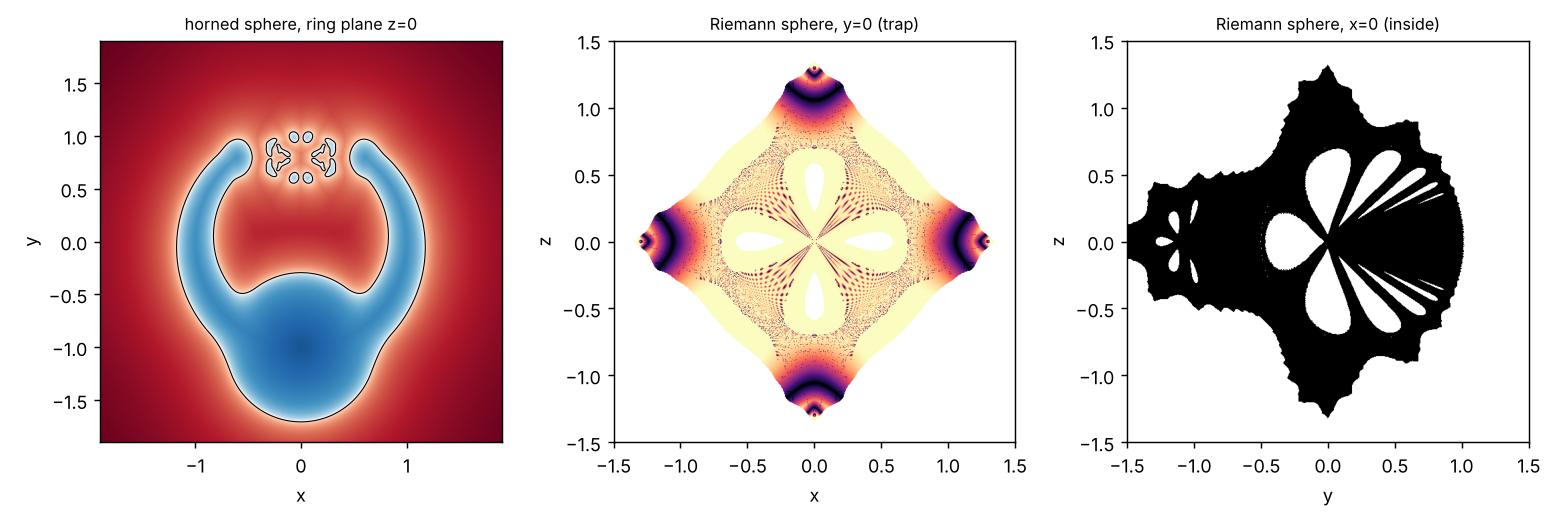
\includegraphics[width=\linewidth]{riemann_horned_slices.png}
\caption{Left: the horned sphere in its ring plane $z=0$, coloured by signed distance (blue inside, red outside, black: the surface); the small islands between the horn tips are
cross-sections of next-generation rings.  Middle: the Riemann sphere at $y=0$ by orbit trap.  Right: the same map at $x=0$, an inside/outside mask.}
\label{fig:riemann_horned_slices}
\end{figure}

\begin{figure}[t]
\centering
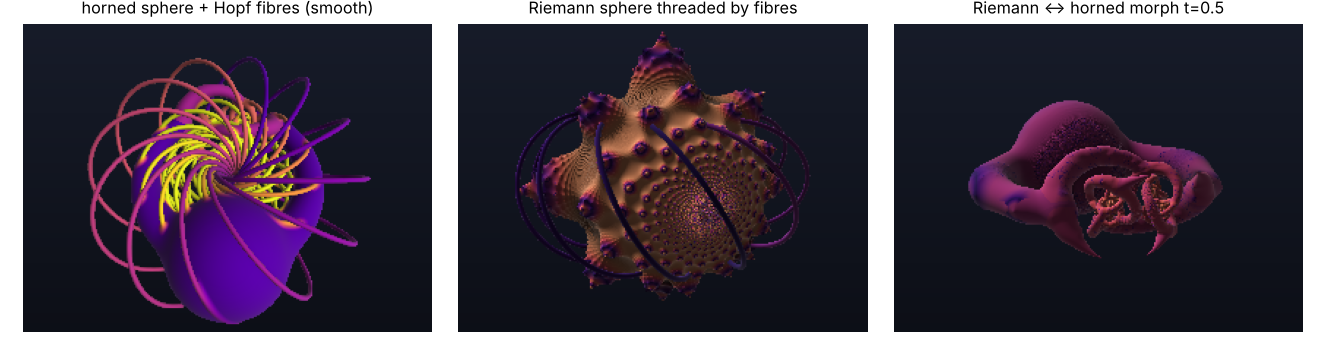
\includegraphics[width=\linewidth]{riemann_horned_mix.png}
\caption{Fields compose.  Left: the horned sphere smooth-unioned with Hopf fibres (three latitudes of twelve fibres, scaled by $0.45$).  Middle: the Riemann sphere united with fibres scaled by $0.35$.
Right: the linear blend $t=\tfrac12$ of the Riemann sphere and the horned sphere, an average of the two distance estimates and so a morph, not a meaningful intermediate shape.}
\label{fig:riemann_horned_mix}
\end{figure}

\section{The horned sphere as a recursive distance field}
\label{sec:horned}

\subsection{Construction}

Let the \emph{ring} $\mathcal R_g$ be the unit circle in the $xy$ plane with the arc $|\varphi|<g$ removed, $\varphi=\operatorname{atan2}(y,x)$.  Its two cut ends are the \emph{tips}
$T_\pm=(\cos g,\pm\sin g,0)$.  A tube of radius
\begin{equation}
\tau(\varphi)=t\,s^{\,a(\pi-|\varphi|)/(\pi-g)},\qquad |\varphi|\in[g,\pi],
\end{equation}
surrounds it, with round caps at the tips: $t$ at the back $\varphi=\pi$, narrowing to $t s^{a}$ at the tips; for $a=1$ this equals the back thickness of a child ring $s$ times smaller, so the horn runs on unbroken through the fork.
Two children are hung from the tips by similarity maps $F_k(l)=t_k+s\,M_k\,l$ with $M_k\in SO(3)$, $k=a,b$: the child's back sits on a tip.  The construction
recurses, so a ring at generation $m$ is $F_{k_1}\circ\dots\circ F_{k_m}(\mathcal R_g)$ with scale $s^m$.  Alexander's horned sphere is obtained when the two children clasp like chain links.
In ray's parametrisation the gap is set by $\sin g=\kappa s$ with $\kappa$ the \code{clasp} parameter, and the children are turned by $\beta$ (\code{turn}) from the parent's plane for one child and $\beta+90^\circ$
for the other.  The rest of this section uses only that the maps are rotations with scale $s$, and so applies to any pair placement, as used in \cref{sec:hopftree}.

\begin{figure}[t]
\centering
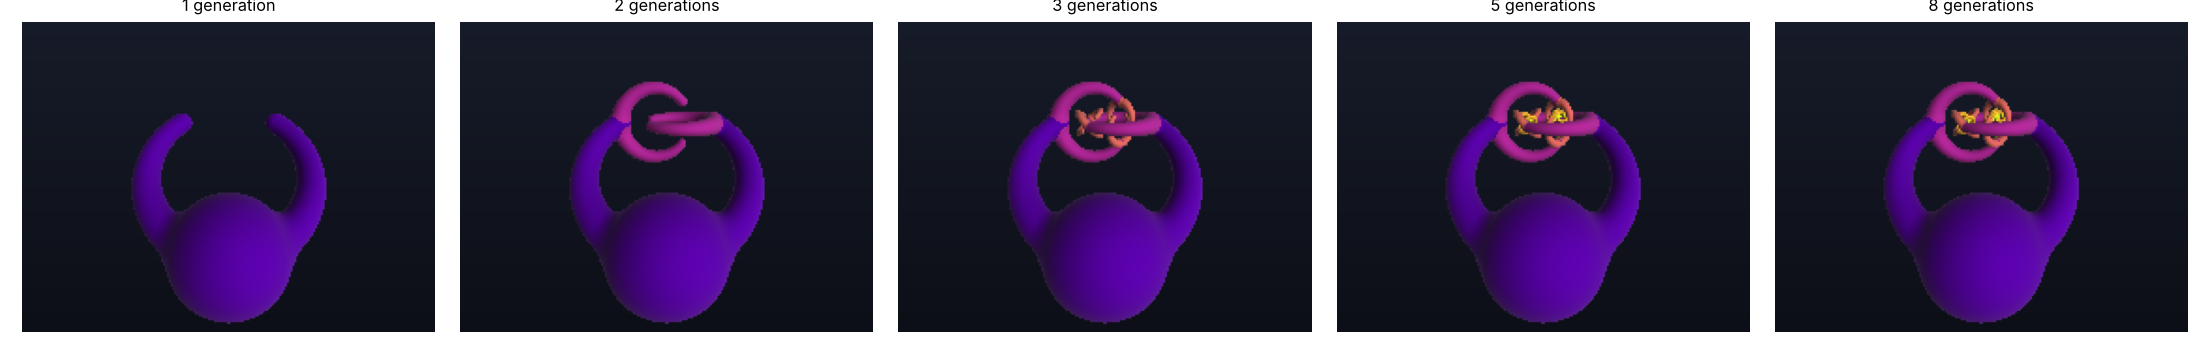
\includegraphics[width=\linewidth]{horned_generations.png}
\caption{The horned sphere with 1, 2, 3, 5 and 8 generations, seen from above.  Each added generation puts two smaller clasped rings on the tips of every ring of the previous one.}
\label{fig:generations}
\end{figure}

\subsection{An exact, order-independent distance}

Let $d_v(P)=s^{m}\,d_{\mathcal R}(F_v^{-1}P)$ be the distance to the tapered tube of ring $v$ at generation $m$, in world units, and $p(v)$ the parent.  With the smoothing width $k_v=\beta_f\,t\,s^{m}$
($\beta_f$ the fillet parameter \code{blend}) define
\begin{equation}
D(P)=\min_{v}\ \smin\!\bigl(d_{p(v)}(P),\,d_v(P);\,k_v\bigr),\qquad d_{p(\text{root})}\equiv+\infty,
\label{eq:horned_de}
\end{equation}
with the root additionally smooth-unioned with a ball.  Each ring is filleted against its parent only.  This is the design that matters: the term for $v$ depends on $v$ and $p(v)$ and nothing else, so $D$ does not
depend on the order in which rings are visited.  A depth-first search that visits the nearer child first, and a level-by-level vectorised search over all sample points
therefore compute the same function.  It is not obvious that the \emph{pruned} versions also agree, because pruning compares against a running minimum; this is the content of the next two statements.

\begin{lemma}\label{lem:smin}
Let $k>0$, $m\in\R$, $a\ge m$ and $b\ge m+k$.  Then $\smin(a,b;k)\ge m$.  (The same holds with $a$ and $b$ exchanged.)
\end{lemma}
\begin{proof}
If $|a-b|\ge k$ then $\smin=\min(a,b)\ge m$.  Otherwise let $u=|a-b|<k$ and $x=k-u\in(0,k]$.  If $a\le b$ then $a\ge b-u\ge m+x$ and $\smin=a-x^2/4k\ge m+x-x^2/4k\ge m$.
If $a>b$ then $\smin=b-x^2/4k\ge m+k-k/4>m$.
\end{proof}

\begin{proposition}\label{prop:prune}
Let $w$ be a ring and $b_w(P)$ a lower bound on $d_u(P)$ for $w$ and all its descendants $u$, and let $\mathrm{best}\le d_{p(w)}(P)$ be a value that is at most the term of every ring already
visited.  If $b_w\ge \mathrm{best}+k_w$, no ring of the subtree of $w$ lowers the minimum below $\mathrm{best}$.
\end{proposition}
\begin{proof}
For $u=w$ apply \cref{lem:smin} with $a=d_{p(w)}\ge\mathrm{best}$ and $b=d_w\ge \mathrm{best}+k_w$.  For a proper descendant $u$ both arguments are at least $b_w\ge\mathrm{best}+k_w\ge\mathrm{best}+k_u$, since $k_u\le k_w$, so $\smin\ge\min-k_u/4\ge\mathrm{best}$.
\end{proof}

The search keeps, for every sample point, the running minimum $\mathrm{best}$ and re-checks the bound when a ring is visited, so $\mathrm{best}$ only decreases and \cref{prop:prune} applies at each check.  The result is therefore \emph{exactly} the minimum \eqref{eq:horned_de} over all rings to the chosen depth, not an approximation to it.
The bound $b_w$ used is the distance to the torus of the thickest tube, $\sqrt{(\sqrt{x^2+y^2}-1)^2+z^2}-t$, together with a ball about the ring's centre that contains all descendants.  It is a valid lower bound because the tapered tube lies inside that torus and the descendants inside the ball (by construction, and tested).


\section{Circle families and linking numbers}
\label{sec:linking}

Both the horned sphere's ring tree and the Hopf fibres are families of circles in $\R^3$.  We expose both as lists of polylines and as a capsule network (\code{FiberNetwork}), a union of capsules usable as a field.  For the tree, the open arcs with the tapered radii form a network whose distance equals the tree's, with fillet and ball turned off, up to the polyline's chord error (tested).

\paragraph{Linking numbers of polylines.}
For two disjoint closed oriented curves,
\begin{equation}
\Lk(A,B)=\frac1{4\pi}\oint\!\oint \frac{(a-b)\cdot(da\times db)}{|a-b|^3}.
\end{equation}
For polylines we evaluate this at segment midpoints,
\begin{equation}
\Lk(A,B)\approx\frac1{4\pi}\sum_{i,j}\frac{(\Delta a_i\times\Delta b_j)\cdot(m_i-m'_j)}{|m_i-m'_j|^3}.
\end{equation}
The result is close to an integer only when the segments are short compared with the gap between the curves, so the pair is densified until the segments are at most half the (refined) gap.  Rings are completed across their cut, since the cut is a feature of the tube, not of the centre circle.

\paragraph{Touching pairs.}
In both families some pairs of circles \emph{touch}: a child's back sits on its parent's tip, so the two closed circles share a point.  The Gauss integral of curves that share a point is not an integer and has no meaning as a linking number; we observed values such as $\pm0.69$ and $\pm0.50$ there.  Such pairs must be excluded, not rounded.
An earlier version of our code detected touching pairs from the polyline distance alone, with a tolerance of $5\%$ of the longest segment.  For the smallest rings the polylines can miss the shared point by a few chord errors, which exceeded the tolerance; those pairs were rounded to $\pm1$ and counted as links, inflating one of our results (\cref{sec:hopftree}).  The code now marks every parent--child pair as touching by construction and the tests check it.

\begin{figure}[t]
\centering
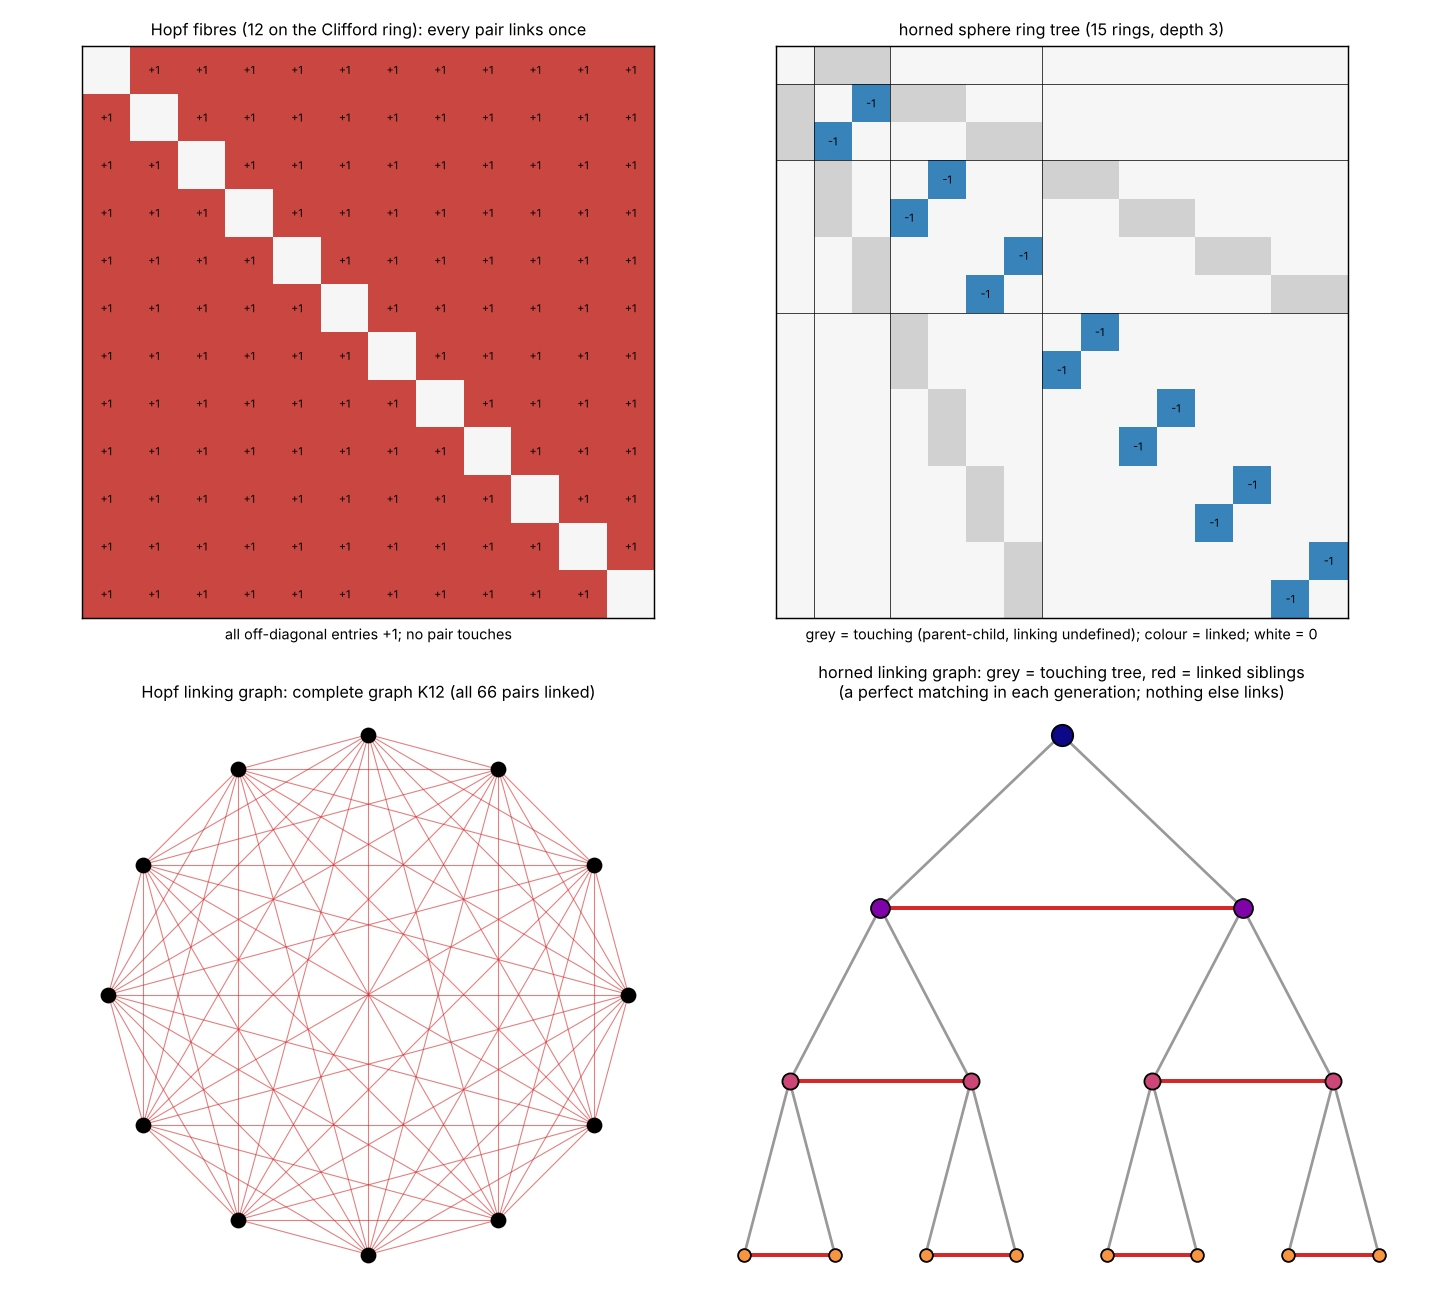
\includegraphics[width=0.88\linewidth]{linking_graphs.png}
\caption{Linking matrices and graphs.  Top left: 12 Hopf fibres on the Clifford torus: every pair links with sign $+1$.  Top right: the horned sphere's ring tree to depth 3 (15 rings): grey marks parent--child pairs, which touch; the only linked pairs are siblings, with sign $-1$.
Bottom: the same as graphs: $K_{12}$ for the fibres, and for the horned tree a perfect matching of siblings in each generation.}
\label{fig:linking_graphs}
\end{figure}

\paragraph{Results.}
\begin{enumerate}[leftmargin=*,itemsep=2pt]
\item \emph{Hopf fibres.}  Twelve fibres on one torus: all $66$ pairs have $\Lk=+1$, none touch, the largest deviation from an integer is $7\times10^{-5}$.  The linking graph is the complete graph $K_{12}$.
\item \emph{Horned sphere.}  At depth 3 (15 rings) 14 pairs touch, the parent--child pairs, and exactly 7 pairs are linked, all siblings, all with $\Lk=-1$.  At depth 4 (31 rings): 30 touching and 15 linked, again exactly the sibling pairs, $\Lk=-1$.
At depth $D$ the number of sibling pairs is $2^D-1$.  No other pair links.  The sibling clasp stays a link for all turn angles $\beta$ in $[0^\circ,90^\circ]$ at the default parameters (\cref{fig:horned_linking}).  The deviation from an integer is below $0.012$ throughout.
\end{enumerate}
The sign is a matter of orientation convention (all rings are oriented by the same parametrisation in right-handed frames); only the pattern, not the sign difference between the two families, should be read from \cref{fig:linking_graphs}.

\begin{figure}[t]
\centering
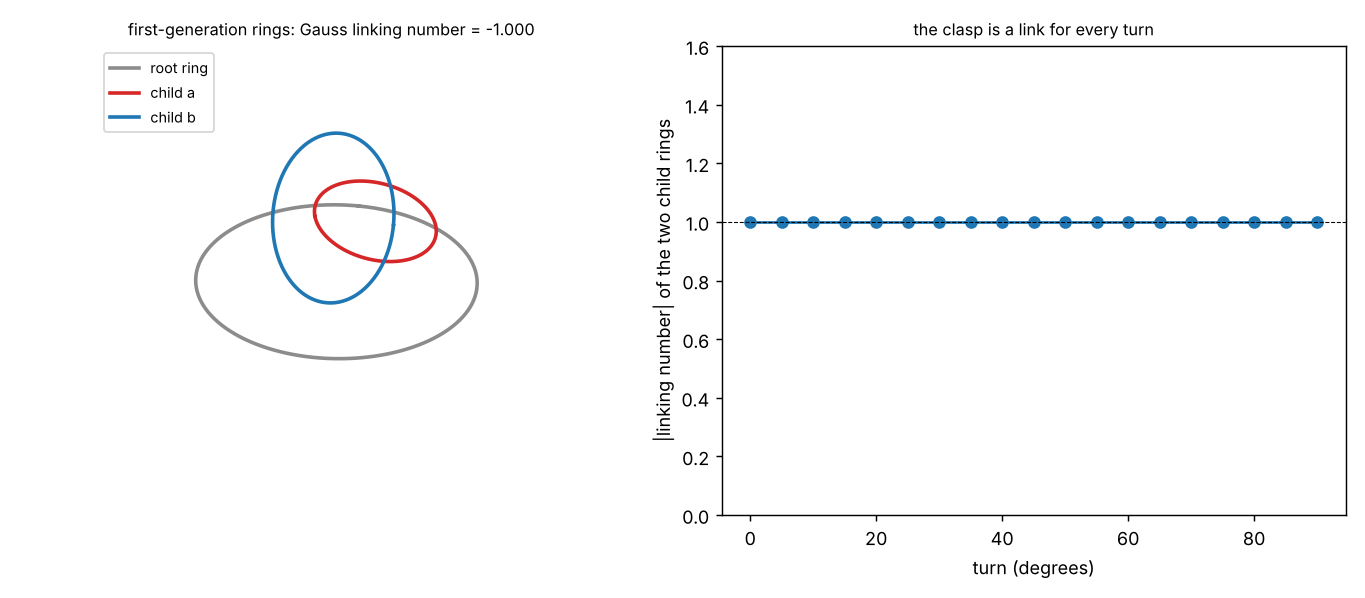
\includegraphics[width=0.8\linewidth]{horned_linking.png}
\caption{Left: the root ring and its two first-generation children as closed circles.  Right: the absolute linking number of the two children against the \code{turn} parameter.}
\label{fig:horned_linking}
\end{figure}

\section{Hopf-paired trees}
\label{sec:hopftree}

\subsection{Construction}

The horned sphere places its two children by hand (\code{clasp} and \code{turn}).  We instead place them as two fibres of the Hopf fibration.
Let the fibre over the base point with Hopf coordinates $(\eta,\phi)$ be
$\gamma(t)=(\cos\eta\,e^{it},\ \sin\eta\,e^{i(t+\phi)})$ and $\sigma(x)=(x_1,x_2,x_3)/(1-x_4)$ the stereographic projection.  Take $\eta=\pi/4$ (the Clifford torus) and $\phi\in\{0,\pi\}$, two antipodal points of the equator of $\Sph^2$.
Their images are two circles of equal radius.  Normalised to radius 1, their centres are at distance $1/\sqrt2$ from the $z$ axis on opposite sides, their planes are perpendicular, they have $\Lk=+1$ (computed: $1.000002$), and the second is the first turned by a half turn about the $z$ axis.  This is the \emph{Hopf pair}.

To hang the pair from the tips of a parent ring we choose one \emph{back point} on each circle, $p_a$ on the first and $p_b$ its half-turn image on the second, parametrised by an angle $\psi$ around the first circle, with $\psi=0$ the point nearest the axis.
Let $\rho(\psi)$ be the distance of $p_a$ from the axis; it ranges over $[1-1/\sqrt2,\ 1+1/\sqrt2]=[0.293,\,1.707]$.  The two back points are $2\rho$ apart, and we send them to the tips $T_\pm$, which are $2\sin g$ apart.  A similarity of scale $s$ does this if and only if
\begin{equation}
\sin g=s\,\rho(\psi),
\label{eq:hopf_gap}
\end{equation}
and so $s\rho<1$, and we reject $s\rho>0.95$.  The similarity sends the pair's half-turn axis to the parent's $x$ axis and $p_a,p_b$ to $T_+,T_-$.  Two discrete choices remain: $\text{hang}=\pm1$, the two placements related by a half turn of the pair about the line through the tips, and $\text{hand}=\pm1$, the chirality.
In effect the fibration fixes what the horned sphere leaves free: the gap $g$ (through \cref{eq:hopf_gap}), and the mutual orientation of the children, so \code{clasp} and \code{turn} disappear.  The free parameters are $s$, $\psi$, \text{hang} and \text{hand}.  We call the resulting field the \emph{Hopf tree}; its distance estimate is that of \cref{sec:horned} with these child maps, and a test confirms that every sibling pair, mapped back through the inverse similarity and inverse stereographic projection, is a pair of fibres over antipodal base points, also at depth 2.
Scans are consistent with the symmetry $(\psi,\text{hang})\leftrightarrow(360^\circ-\psi,-\text{hang})$.

\begin{figure}[t]
\centering
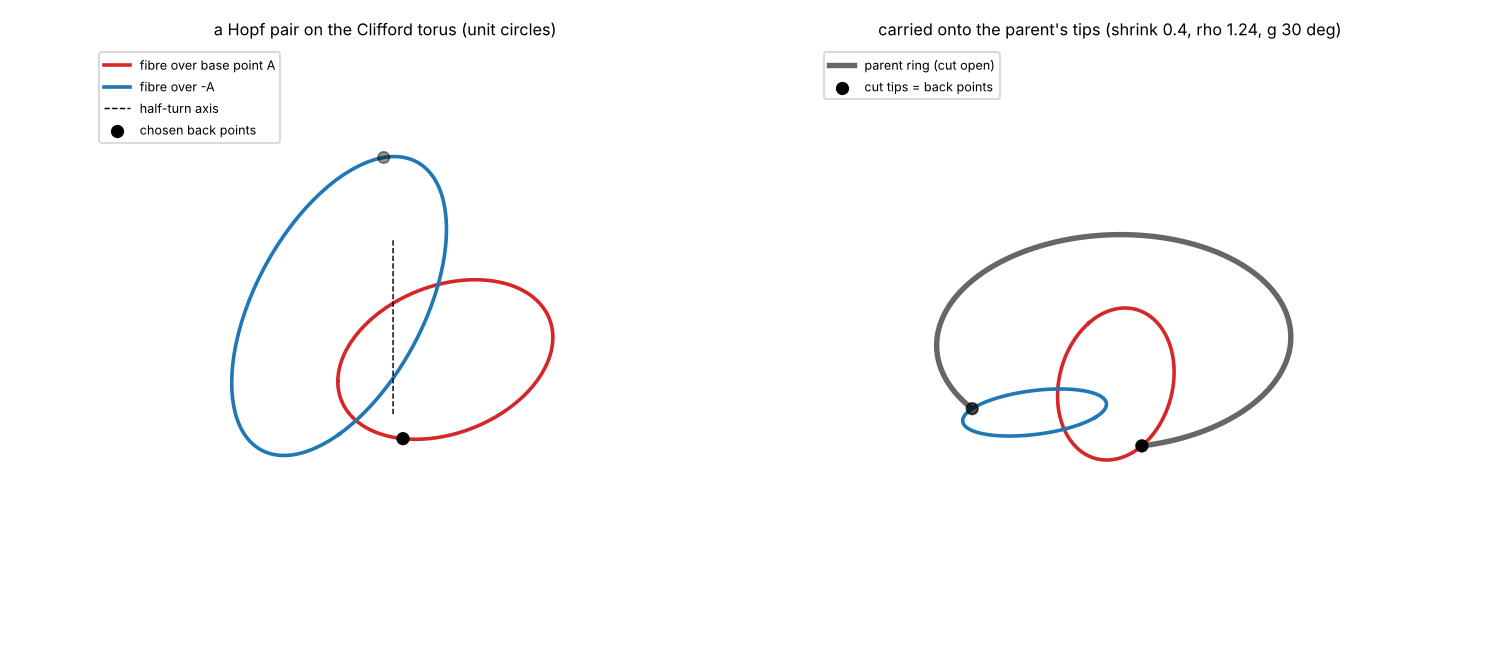
\includegraphics[width=\linewidth]{hopf_tree_pair.png}
\caption{Left: a Hopf pair on the Clifford torus (unit circles), with the half-turn axis and the chosen back points.  Right: the pair carried onto the cut tips of a parent ring (for $s=0.4$, $\psi=110^\circ$: $\rho=1.24$, $g=30^\circ$).}
\label{fig:hopf_pair}
\end{figure}

\subsection{Self-similarity of the link graph}

\begin{proposition}\label{prop:selfsim}
Let $F_a,F_b$ be orientation-preserving similarities and $\mathcal R$ a closed curve.  For a word $\pi$ in $\{a,b\}$ write $F_\pi$ for the composition and let $X$ and $X\pi$ be the rings $F_X(\mathcal R)$ and $F_XF_\pi(\mathcal R)$.  Then $\Lk(X,X\pi)=\Lk(\mathcal R,F_\pi\mathcal R)$ whenever the curves are disjoint; i.e.\ the linking number between a ring and its descendant at a given relative position does not depend on the ring.
\end{proposition}
\begin{proof}
An orientation-preserving similarity of $\R^3$ preserves linking numbers.
\end{proof}

All the child maps in \code{fractalkit} are rotations times a scale ($\det M_k=+1$ for the horned sphere, and for the Hopf tree for both values of \text{hang}), so the proposition applies.  It explains why the linking graphs found below are the same at every generation: what a ring links among its descendants is decided once, at the root.  It does not decide which pairs of non-nested rings link, and for those we rely on computation.

\subsection{Results}

We computed the linking graphs of the completed rings for $s=0.4$ and \text{hang}$=+1$, scanning $\psi$.  As a measure of how thick the tubes can be we use $t_{\max}$: the largest value of the tube parameter $t$ such that the untapered tubes around the open arcs of every pair of non-adjacent rings do not overlap, i.e.\
$\min_{u,v}\mathrm{dist}(\text{arc}_u,\text{arc}_v)/(s_u+s_v)$ over pairs that are not parent and child.  The taper only narrows tubes, so this is conservative.  For comparison, the horned sphere at default parameters has $t_{\max}=0.252$ (depths 3 and 4).

\begin{table}[t]
\centering\small
\begin{tabular}{@{}rrrrrrl@{}}
\toprule
$\psi$ & $\rho$ & $g$ & linked & non-sibling & $t_{\max}$ & signs \\ \midrule
$60^\circ$  & 0.646 & 15.0$^\circ$ & 7  & 0  & 0.293 & $+1$ \\
$110^\circ$ & 1.242 & 29.8$^\circ$ & 7  & 0  & 0.156 & $+1$ \\
$130^\circ$ & 1.455 & 35.6$^\circ$ & 7  & 0  & 0.027 & $+1$ \\
$150^\circ$ & 1.612 & 40.2$^\circ$ & 23 & 16 & 0.019 & $\pm1$ \\
$180^\circ$ & 1.707 & 43.1$^\circ$ & 31 & 24 & 0.047 & $\pm1$ \\
$205^\circ$ & 1.641 & 41.0$^\circ$ & 13 & 6  & 0.104 & $\pm1$ \\
$215^\circ$ & 1.579 & 39.2$^\circ$ & 13 & 6  & 0.210 & $\pm1$ \\
$220^\circ$ & 1.542 & 38.1$^\circ$ & 13 & 6  & 0.250 & $\pm1$ \\
$222^\circ$ & 1.525 & 37.6$^\circ$ & 7  & 0  & 0.267 & $+1$ \\
$240^\circ$ & 1.354 & 32.8$^\circ$ & 7  & 0  & 0.293 & $+1$ \\ \bottomrule
\end{tabular}
\caption{Hopf tree, $s=0.4$, hang $=+1$, depth 3 (15 rings, 7 sibling pairs).  ``Linked'' counts linked pairs among non-touching pairs; $t_{\max}$ is defined in the text.}
\label{tab:regimes}
\end{table}

\begin{figure}[t]
\centering
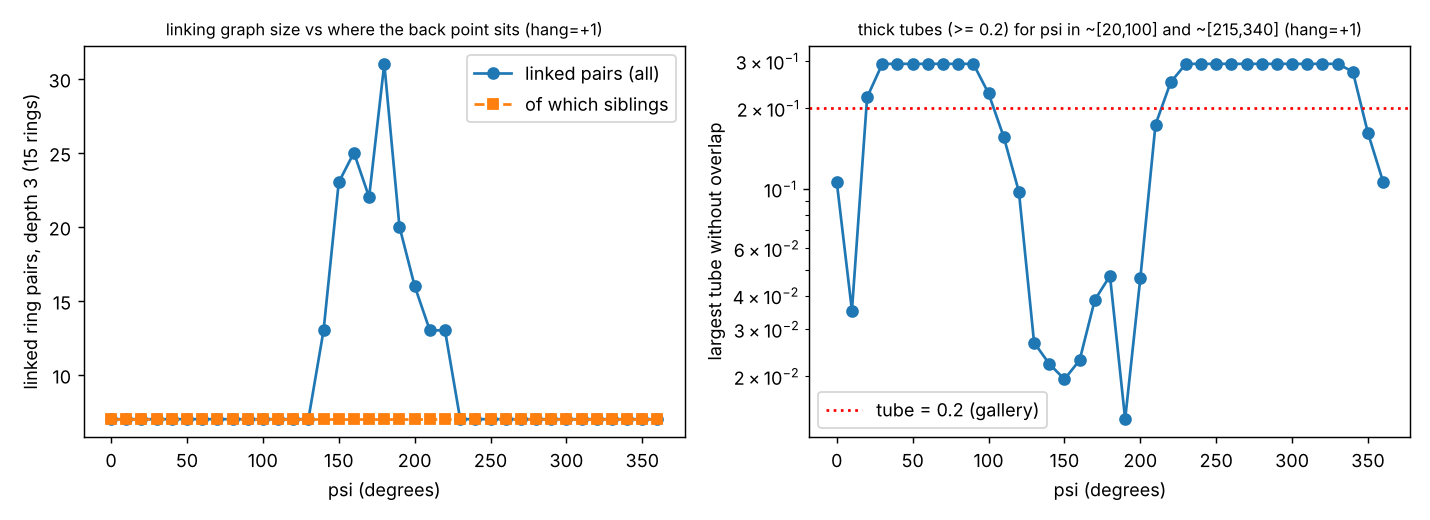
\includegraphics[width=\linewidth]{hopf_tree_phase.png}
\caption{Left: number of linked ring pairs at depth 3 against $\psi$ (steps of $10^\circ$); the sibling count is constant at 7.  Right: $t_{\max}$ (log scale) against $\psi$; the dotted line is the tube thickness $0.2$ used in the renderings.}
\label{fig:phase}
\end{figure}

Three regimes appear (\cref{tab:regimes}, \cref{fig:phase}).

\begin{enumerate}[leftmargin=*,itemsep=2pt]
\item \emph{Sibling-only} (for $\psi\lesssim130^\circ$ and $\psi\gtrsim222^\circ$): the linking graph is that of the horned sphere, a perfect matching of siblings, here with sign $+1$ in our convention.  Tubes with $t\ge0.2$ are possible for $\psi$ from about $20^\circ$ to $100^\circ$ and from about $222^\circ$ to $340^\circ$.
\item \emph{Thin and rich} ($130^\circ<\psi<202^\circ$): many more links (up to 31 of the 91 non-touching pairs at depth 3), but $t_{\max}\le0.05$, so the tubes are wire-like.  At $\psi=180^\circ$, which is a horned sphere with a Hopf clasp (\cref{sec:clasp}), and depth 4, 123 of the 421 non-touching pairs are linked, but 14 pairs beyond the parent--child ones touch, so the centre-lines intersect and this is no longer an embedded tree.
\item \emph{Thick and rich} ($202^\circ\le\psi\le221^\circ$, checked at $1^\circ$ steps): the tubes can be thick ($t_{\max}=0.10$ at $205^\circ$, $0.21$ at $215^\circ$, $0.25$ at $220^\circ$) and there are links beyond the siblings, following a rule.
\end{enumerate}

\begin{observation}[grandchild rule]\label{obs:rule}
For $s=0.4$, hang $=+1$ and $202^\circ\le\psi\le221^\circ$ the linked non-touching pairs of the Hopf tree are exactly: each sibling pair, and for every ring $X$ with grandchildren in the tree, the pairs $\{X,\,b(a(X))\}$ with $\Lk=-1$ and $\{X,\,b(b(X))\}$ with $\Lk=+1$, where $a(\cdot),b(\cdot)$ are the first and second child.
\end{observation}

The number of such non-sibling links at depth $D$ is $2(2^{D-1}-1)$: 6 at depth 3 and 14 at depth 4.  We checked \cref{obs:rule} on the full linking matrix at depth 3 for every integer $\psi$ from $196^\circ$ to $235^\circ$: it holds exactly for $202^\circ$--$221^\circ$ and fails outside.  We checked it at depth 4 (31 rings, with 30 touching pairs and no other) for $\psi=205^\circ$, $215^\circ$ and $220^\circ$; the observed non-sibling pairs and signs equal the prediction in all cases (the deviation from integers is at most $0.012$).  At $215^\circ$ and $220^\circ$ the clearance at depth 4 is $t_{\max}=0.21$ and $0.25$, the same as at depth 3.
It is an observation, not a theorem: \cref{prop:selfsim} says that the links of a ring with its descendants repeat from ring to ring, which accounts for the pattern repeating by generation, but the values at the root, and the absence of other links, come from computation.  At $222^\circ$ the non-sibling links have disappeared although the clearance is still thick ($0.267$).  A linking number can change only when two of the completed circles cross, and such a crossing can happen in the removed cut, where the open arcs that $t_{\max}$ measures do not meet; we did not locate the crossings.
\Cref{fig:rule} shows the rule at $215^\circ$ and \cref{fig:linking_mats} the matrices of the horned sphere and three Hopf trees.

\begin{figure}[t]
\centering
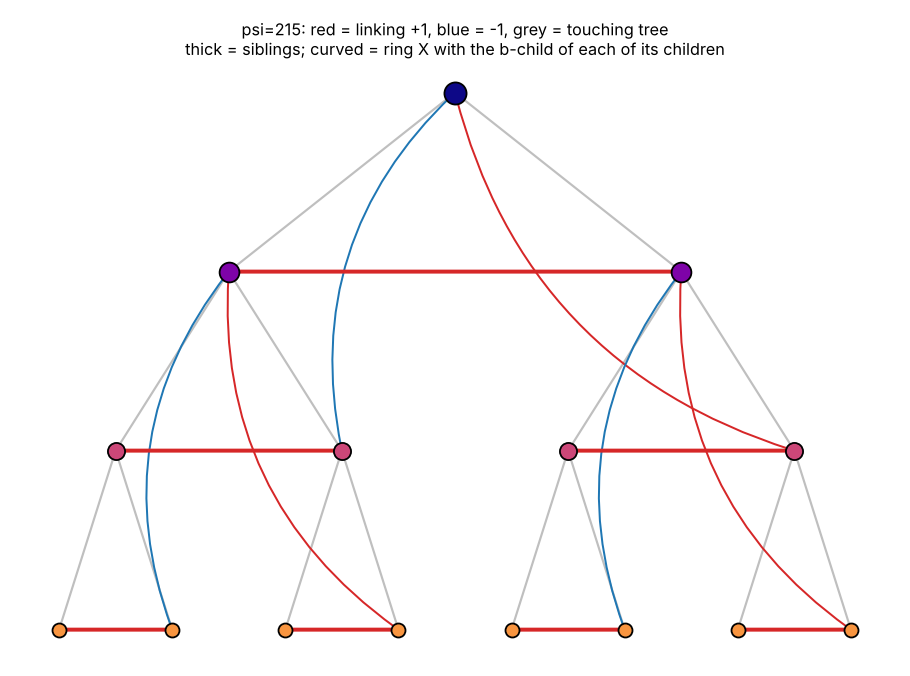
\includegraphics[width=0.72\linewidth]{hopf_tree_graph.png}
\caption{The linking graph of the Hopf tree at $\psi=215^\circ$, depth 3.  Grey: touching parent--child pairs.  Thick red: siblings.  Curved: each ring with the second child of each of its children (red $+1$, blue $-1$).}
\label{fig:rule}
\end{figure}

\begin{figure}[t]
\centering
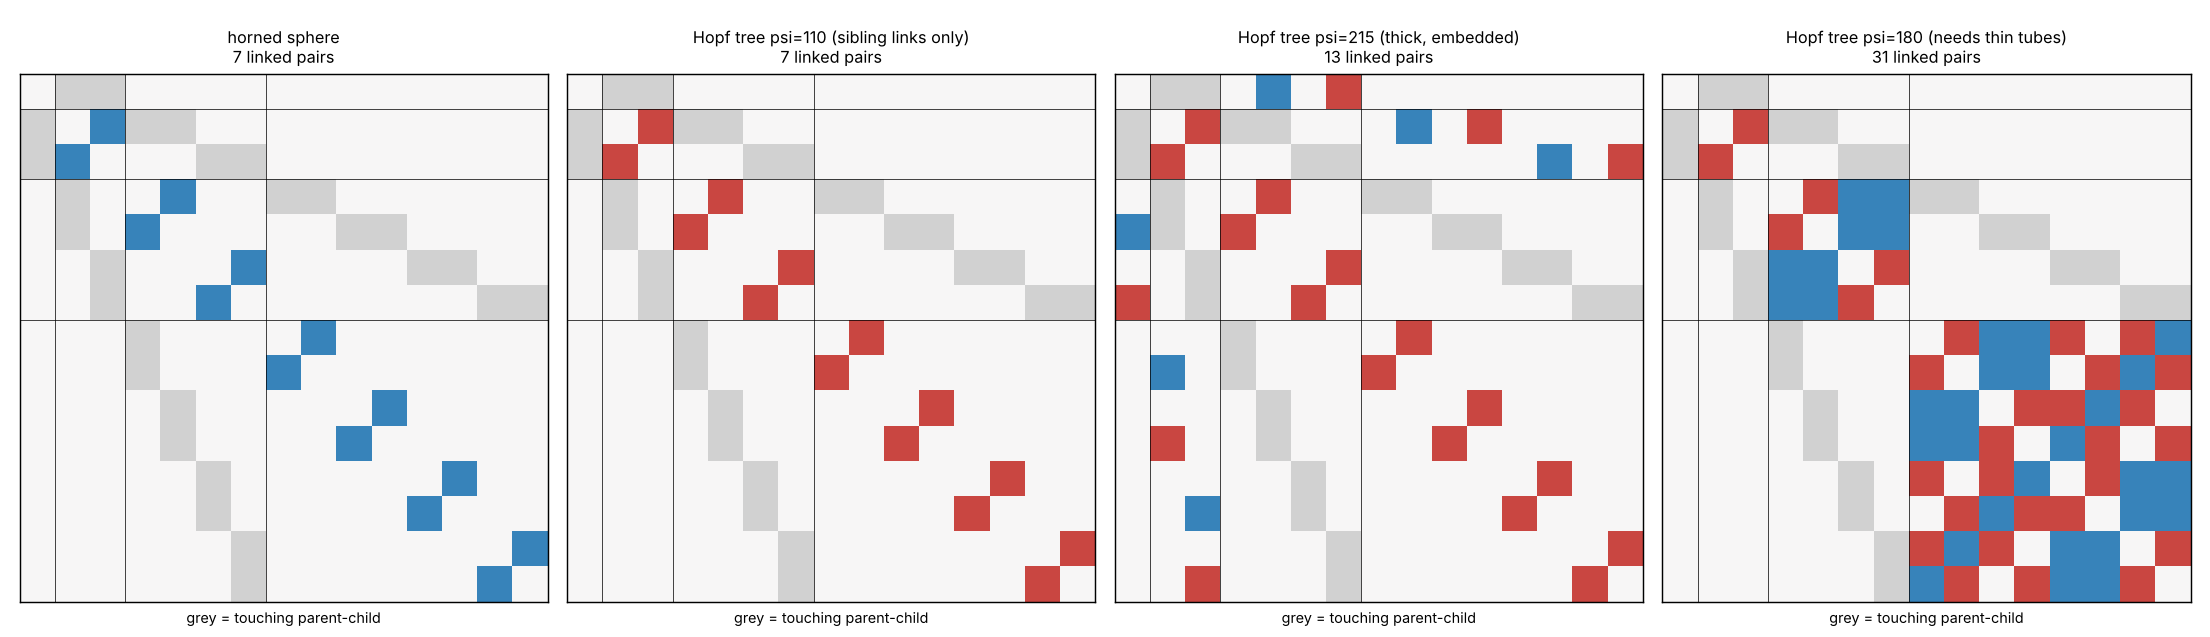
\includegraphics[width=\linewidth]{hopf_tree_linking.png}
\caption{Linking matrices at depth 3: the horned sphere (7 linked pairs, sign $-1$), the Hopf tree at $\psi=110^\circ$ (7, the same graph), at $215^\circ$ (13, the grandchild rule), and at $180^\circ$ (31, thin tubes only).  Grey: touching.  The block boundaries mark generations.}
\label{fig:linking_mats}
\end{figure}

\begin{figure}[t]
\centering
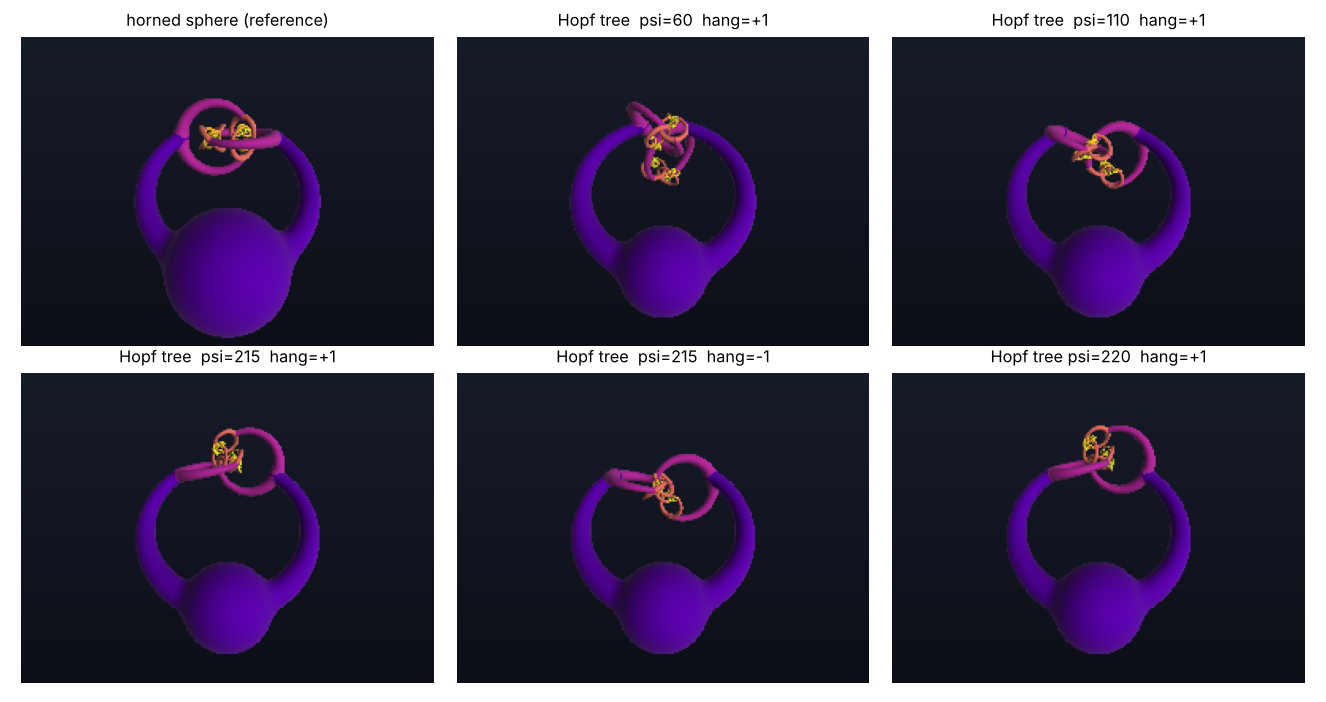
\includegraphics[width=\linewidth]{hopf_tree_gallery.png}
\caption{Distance-field renderings at 7 generations with tube $0.2$: the horned sphere for reference, and Hopf trees at $\psi=60^\circ,110^\circ,215^\circ,220^\circ$ with hang $=+1$ and at $215^\circ$ with hang $=-1$.  At this resolution the finest generations are not visible.}
\label{fig:gallery_hopf}
\end{figure}

\section{The clasp as a M\"obius object: horned spheres, the oloid and the Hopf fibration}
\label{sec:clasp}

The companion repository \code{HopfFibration}~\ref{hopffibration} studies chains of round circles, the cores of Antoine's necklace~\cite{wiki_antoine,schwartz2022}, against Hopf fibres, and compares the two-circle clasp with the oloid~\cite{wiki_oloid}.  Its tools apply directly to the clasp of the horned sphere of \cref{sec:horned}, and give a one-parameter picture of what \code{clasp} does.  We reproduce its Lorentz-model invariant in \code{fractalkit} (\code{circle\_moebius\_invariants}) and check the results below against the companion's own implementation.

\subsection{Invariants of a pair of circles}

A round circle in $\R^3\cup\{\infty\}$ is, in the Lorentz model $\R^{4,1}$ with metric $\eta=\operatorname{diag}(1,1,1,1,-1)$, the 2-plane $W$ of the spheres through it: it is spanned by a plane through the circle and a sphere having it as equator, both unit spacelike.  For circles with frames $W_1,W_2$ the singular values $s_1\ge s_2$ of the Gram matrix $W_1\eta W_2^{\top}$ are invariant under M\"obius maps.  When both are below 1 the pair is M\"obius-equivalent to two great circles of $\Sph^3$ with principal angles $\theta_i=\arccos s_i$, and it is a pair of Hopf fibres exactly when the great circles are Clifford parallel, $s_1=s_2$~\ref{hopffibration}.

\begin{proposition}\label{prop:clasp}
Let two circles of radius $r$ lie in perpendicular planes, with the line joining their centres, at distance $d$, lying in both planes.  Then $(s_1,s_2)=(|1-d^2/2r^2|,\,0)$.
\end{proposition}
\begin{proof}
Scale to $r=1$ and place $A$ in $z=0$ with centre $0$ and $B$ in $y=0$ with centre $(d,0,0)$.  Writing frames as (plane, sphere),
\begin{align*}
W_A&=\{(0,0,1,0,0),\ (0,0,0,-1,0)\},\\
W_B&=\{(0,1,0,0,0),\ (d,0,0,\tfrac{d^2-2}{2},\tfrac{d^2}{2})\}.
\end{align*}
The Gram matrix has one nonzero entry, $(0,0,0,-1,0)\,\eta\,(d,0,0,\tfrac{d^2-2}{2},\tfrac{d^2}{2})^{\top}=1-\tfrac{d^2}{2}$.
\end{proof}

For the two children of a ring in the horned sphere, the radius is $s$ and the centres are $2\,\mathrm{off}=2s(\kappa-1)$ apart, so $d/r=2(\kappa-1)$ and the first invariant is
\begin{equation}
s_1(\kappa)=\bigl|1-2(\kappa-1)^2\bigr|,\qquad s_2=0,
\label{eq:clasp_s1}
\end{equation}
where $\kappa$ is the \code{clasp} parameter.  The children's planes are perpendicular, and the centre line lies in both, for every $\kappa$ and every \code{turn} we tried; we checked this numerically, and checked \cref{eq:clasp_s1} against the companion's implementation at six values of $\kappa$ and two turns, to $10^{-15}$ (\cref{fig:clasp}, left).  Three consequences:

\begin{itemize}[leftmargin=*,itemsep=2pt]
\item $s_1=0$ exactly at $\kappa=1+1/\sqrt2\approx1.7071$.  The clasp is then a Hopf pair over antipodal base points, the same pair as in \cref{sec:hopftree}, and the \code{turn} parameter drops out of the invariants.
\item $s_1=\tfrac12$ at $\kappa=\tfrac32$ (and again at $\kappa=1+\sqrt3/2\approx1.866$): the clasp is then M\"obius-equivalent to the pair of circles of the oloid, whose principal angles are $60^\circ$ and $90^\circ$, so it is $30^\circ$ from a Hopf pair on the second sphere factor~\cite{wiki_oloid}.
\item The default $\kappa=1.35$ has $s_1=0.755$, a clasp that is neither.
\end{itemize}
In the language of the companion, the straight chain of circles at $d=\sqrt2\,r$ is the two-circle roller~\cite{wiki_oloid}, and $\kappa=1+1/\sqrt2$ is the value at which the horned sphere's clasp becomes that pair.

\begin{observation}\label{obs:hopf_is_horned}
For $s=0.4$ and $\psi=180^\circ$, the Hopf tree of \cref{sec:hopftree} has the same circles at each generation as the horned sphere with $\kappa=1+1/\sqrt2$ and \code{turn}$=-45^\circ$ or $135^\circ$: with hang and hand both $+1$ the Hausdorff distance between the sampled circles of generations $1,\dots,4$ is $4.5\times10^{-16}$ (all four hang/hand choices agree to $4\times10^{-16}$ through generation 2).
\end{observation}
Both have 31 linked pairs at depth 3.  The ``thin and rich'' member at $\psi=180^\circ$ of \cref{sec:hopftree} is therefore a point of the horned sphere's two-parameter family, reached at the one $\kappa$ where its clasp is a Hopf pair; the Hopf tree for other $\psi$ is not of that form.  This is a numerical equality, not a proof, although at $\psi=\pi$ the back point is the farthest one, so that $\rho=1+1/\sqrt2$ in \cref{eq:hopf_gap} and $\sin g=\kappa s$ with $\kappa=1+1/\sqrt2$, as for the horned sphere.

\subsection{Is the Hopf clasp special for linking?}

One might expect the exact Hopf clasp to be distinguished.  It is not.  \Cref{fig:clasp} (right) counts the linked pairs of the depth-3 horned tree at $s=0.4$, $\text{turn}=45^\circ$ over a range of $\kappa$; \cref{tab:clasp} lists the values.  Sibling pairs link at every $\kappa$ from $1.1$ to $1.9$ (7 pairs); for $\kappa\ge2$ the clasp is open ($d\ge2r$) and the children no longer link.  The default $\kappa=1.35$ and $\kappa=1.5$ have \emph{only} those; the other values have more, in broad bands, from $19$ at $1.2$ to $39$ at $1.8$ and $13$ at $1.9$, with $31$ at the Hopf value.  The clasp invariant $s_1$ does not predict the count: $\kappa=1.1$ ($s_1=0.98$) has $31$ links and $\kappa=1.7$ ($s_1=0.02$) has $33$.  At $\kappa=1.65$ four extra pairs touch, and at $\kappa=2.0$ seven, so those trees are not embedded; the table is silent about whether the tubes at the other $\kappa$ can be made disjoint (we did not compute $t_{\max}$ here).

\begin{table}[t]
\centering\footnotesize
\begin{tabular}{@{}rrrrr@{}}
\toprule
$\kappa$ & $s_1$ & linked & sibling & extra touching \\ \midrule
1.10 & 0.980 & 31 & 7 & 0 \\
1.20 & 0.920 & 19 & 7 & 0 \\
1.35 (default) & 0.755 & 7 & 7 & 0 \\
1.50 (oloid) & 0.500 & 7 & 7 & 0 \\
1.60 & 0.280 & 15 & 7 & 0 \\
1.65 & 0.155 & 25 & 7 & 4 \\
1.70 & 0.020 & 33 & 7 & 0 \\
$1+1/\sqrt2$ (Hopf) & 0.000 & 31 & 7 & 0 \\
1.75 & 0.125 & 33 & 7 & 0 \\
1.80 & 0.280 & 39 & 7 & 0 \\
1.90 & 0.620 & 13 & 7 & 0 \\
2.00 & 1.000 & 0 & 0 & 7 \\
2.20 & 1.880 & 0 & 0 & 0 \\ \bottomrule
\end{tabular}
\caption{The clasp invariant and the linked pairs of the depth-3 horned tree, $s=0.4$, $\text{turn}=45^\circ$.  ``Extra touching'' counts touching pairs other than parent--child.  The 24 values of \code{turn} in steps of $15^\circ$ at $\kappa=1+1/\sqrt2$ give 27 to 39 linked pairs, always with 7 siblings.}
\label{tab:clasp}
\end{table}

\begin{figure}[t]
\centering
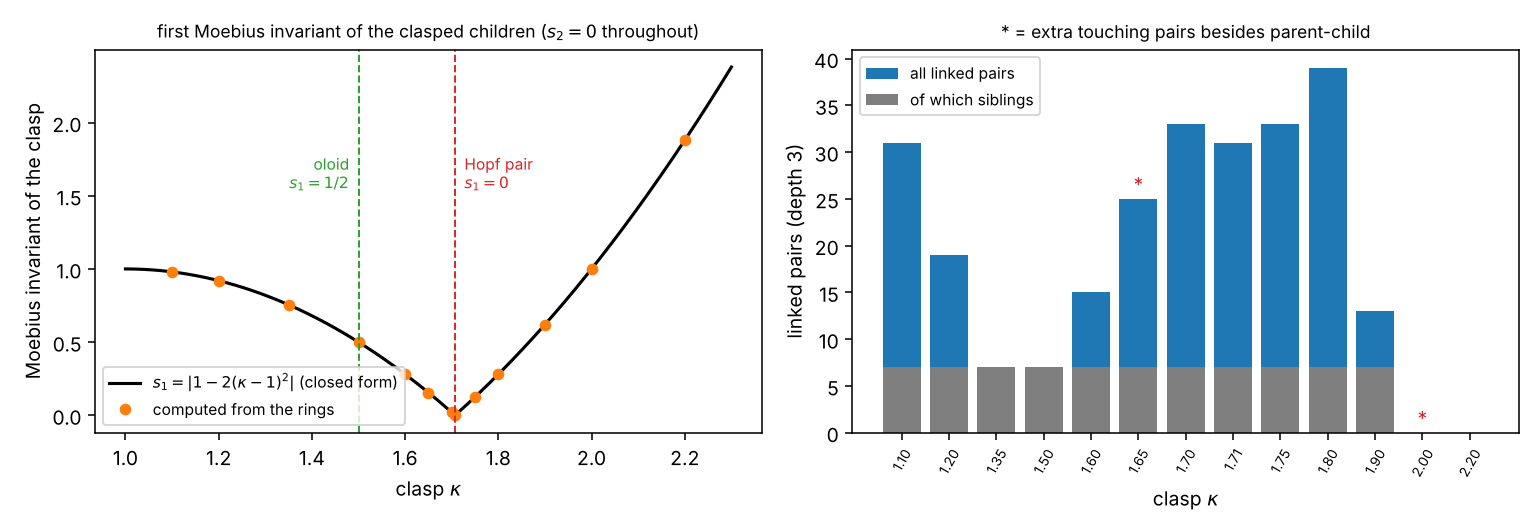
\includegraphics[width=\linewidth]{hopf_clasp.png}
\caption{Left: the first M\"obius invariant of the clasped children against $\kappa$, closed form \cref{eq:clasp_s1} and values computed from the rings ($s_2$ is zero to $10^{-15}$).  The oloid pair is at $\kappa=3/2$ and the Hopf pair at $1+1/\sqrt2$.  Right: linked pairs of the depth-3 tree, with the sibling pairs in grey.}
\label{fig:clasp}
\end{figure}

\subsection{Fibres, necklaces and trees}

We report two contrasting graphs: Hopf fibres link pairwise and so form a complete graph, while a necklace of round circles links only neighbours, a cycle~\ref{hopffibration}; the first is what \cref{sec:linking} found for twelve fibres.  In Antoine's necklace adjacent tori are linked and non-adjacent ones are not~\cite{schwartz2022}, and a necklace needs many links ($K$ large; the notes work with $K\ge20$) so that nested generations stay disjoint~\cite{schwartz2022}.  A ring of the horned sphere has only $K=2$ children, so its ``necklace'' is one clasp, and its graph is sibling pairs.  That is why the non-sibling links of the Hopf tree and of the horned sphere at larger $\kappa$ (\cref{tab:clasp}) have no counterpart in a necklace: they come from circles of different branches, not from adjacent ones.  Conversely, a closed ring of $k$ circles whose every clasp is an exact Hopf pair requires twisting the link planes, with a clasp invariant it observes to equal $\tan(\pi/k)$ for $k=8,12,16,24,32$, and that no single Hopf fibration contains three consecutive circles of a chain~\ref{hopffibration}.

\subsection{ Discussion }

The following are questions raised by these connections.
\begin{enumerate}[leftmargin=*,itemsep=2pt]
\item \emph{Why the Hopf value?}  At $\kappa=1+1/\sqrt2$ the clasp is the two-circle roller, whose centre of mass rolls at constant height~\cite{wiki_oloid}, and it is also an exact Hopf pair.  The companion lists this as an unexplained coincidence~\ref{hopffibration}; \cref{tab:clasp} shows that the count of linked pairs does not single the value out.
\item \emph{Hopf invariant as the linking number.}  The Hopf invariant of a map $\Sph^3\to\Sph^2$ is the linking number of the preimages of two regular values, and torus-knot preimages link $pq$ times for $z_1^p,z_2^q$~\cite{hou2025}; it is the same Gauss integral as \cref{sec:linking}.  Whether the non-sibling links of the Hopf tree correspond to preimages of some map is unknown.
\item \emph{Limit sets.}  Whether the limit set of a Hopf tree is wild is open; the companion proposes testing pearl necklaces whose pearls bound Hopf clasps, as limit sets of Kleinian groups, but notes that no source states that either horned sphere arises that way~\ref{hopffibration}.
\end{enumerate}

\section{Inversion groups: Kleinian groups, pseudo-Kleinian fold}
\label{sec:kleinian}

A Kleinian group is a discrete subgroup of $\mathrm{PSL}(2,\C)$ acting on the Riemann sphere by M\"obius maps; its limit set is the set of accumulation points of an orbit, and a Schottky-type group generated by inversions in disjoint circles has a Cantor set as limit set~\cite{wiki_kleinian}.  The \code{kleinian} formula of ray, Knighty's pseudo-Kleinian, iterates a box fold and an inversion in a sphere, a Mandelbox of scale $1$, and is named for its resemblance to such limit sets.  Both are built from inversions, which suggests asking when the inversions that the horned sphere's rings define \emph{do} generate a discrete group.  We answer this for the ring and its two children.

\subsection{Angles between the equatorial spheres}

Each ring (unit circle, centre $0$) and its two children (radius $s$, centres $(c_g,\pm\mathrm{off},0)$ with $c_g=\sqrt{1-\kappa^2s^2}$ and $\mathrm{off}=s(\kappa-1)$) bounds an \emph{equatorial sphere}, the sphere of the same centre and radius.

\begin{proposition}\label{prop:angles}
The equatorial sphere of the parent meets each child's at angle $\theta_{pc}$ with $\cos\theta_{pc}=\kappa s=\sin g$, and the two children's meet at $\theta_{cc}$ with $\cos\theta_{cc}=1-2(\kappa-1)^2$, which is the Hopf-clasp invariant $\pm s_1$ of \cref{eq:clasp_s1}.
\end{proposition}
\begin{proof}
For spheres of radii $r_1,r_2$ with centres $d$ apart the cosine is $(r_1^2+r_2^2-d^2)/2r_1r_2$.  The parent--child centre distance satisfies $d^2=c_g^2+\mathrm{off}^2=1-s^2(2\kappa-1)$, giving $(1+s^2-d^2)/2s=\kappa s$.  The children are $2s(\kappa-1)$ apart, giving $1-2(\kappa-1)^2$.
\end{proof}
In the Lorentz model the cosine of the angle between two spheres is the inner product of their unit vectors, which is the single nonzero entry of the Gram matrix in the proof of \cref{prop:clasp}; so the clasp invariant $s_1$ is the cosine of the angle between the children's equatorial spheres.  A test checks both cosines and this identification.

\subsection{A family of reflection triangles}

Take the region inside the parent sphere and outside both children.  In the plane of the centres it is a circular triangle: its corners are two parent--child intersection points and the point on the axis where the children meet inside the parent, with angles $\theta_{pc}$ at the first two and $\pi-\theta_{cc}$ at the third (the region lies outside both children there).  Requiring the angles to be $\pi/m,\pi/m,\pi/n$ gives
\begin{equation}
\kappa_n=1+\cos\frac{\pi}{2n},\qquad s_{m}=\frac{\cos(\pi/m)}{\kappa_n},
\label{eq:coxeter}
\end{equation}
so that $s_1=\cos(\pi/n)$.  The first values are $\kappa_2=1+1/\sqrt2$, the Hopf clasp ($s_1=0$), and $\kappa_3=1+\sqrt3/2\approx1.866$, the second of the two $\kappa$ with the oloid's invariant $s_1=\tfrac12$ (\cref{sec:clasp}); $\kappa_n\to2$, tangent children, as $n\to\infty$.  The gap angle is $g=\pi/2-\pi/m$.

Inversion in the three spheres generates a group which, since the triangle is a reflection triangle, satisfies the Coxeter relations $(r_0r_1)^m=(r_0r_2)^m=(r_1r_2)^n=1$.  We verified these numerically for seven pairs $(m,n)$ to $2\times10^{-14}$ at a generic point, while at $s=0.46$ and $0.50$ with $\kappa=\kappa_2$, where $\theta_{pc}$ is not $\pi/m$, the relation fails (error $0.5$).  When $2/m+1/n<1$ the triangle is hyperbolic; the three circles then have a common orthogonal circle $C$ (radius$^2$ positive in every case we computed), and by the classical Poincar\'e polygon theorem the group is discrete with fundamental domain this triangle and limit set $C$.  We did not re-prove this; we checked that the orthogonal circle exists and the figure draws the images of the three circles under all reduced words of length at most $5$ (\cref{fig:reflection}).  (An orbit of random words falling on $C$ is \emph{not} evidence of discreteness: the same happens at the generic $s$, where the group is not discrete, so we do not use it.)

\begin{table}[t]
\centering\small
\begin{tabular}{@{}rrrrrrr@{}}
\toprule
$m$ & $n$ & $\kappa_n$ & $s_m$ & linked pairs & extra touching & note \\ \midrule
5 & 2 & 1.7071 & 0.4739 & 39 & 0 & Hopf clasp \\
6 & 2 & 1.7071 & 0.5073 & 39 & 0 & Hopf clasp \\
7 & 2 & 1.7071 & 0.5278 & 39 & 0 & Hopf clasp \\
4 & 3 & 1.8660 & 0.3789 & 39 & 0 & oloid invariant \\
5 & 3 & 1.8660 & 0.4336 & 13 & 12 & \\
3 & 4 & 1.9239 & 0.2599 & 31 & 4 & \\
4 & 4 & 1.9239 & 0.3675 & 13 & 0 & \\ \bottomrule
\end{tabular}
\caption{Members of the reflection family \cref{eq:coxeter} used as the horned-sphere parameters (\code{shrink} $=s_m$, \code{clasp} $=\kappa_n$, \code{turn} $=45^\circ$), depth 3.  ``Extra touching'': touching pairs besides parent--child.}
\label{tab:coxeter}
\end{table}

\begin{figure}[t]
\centering
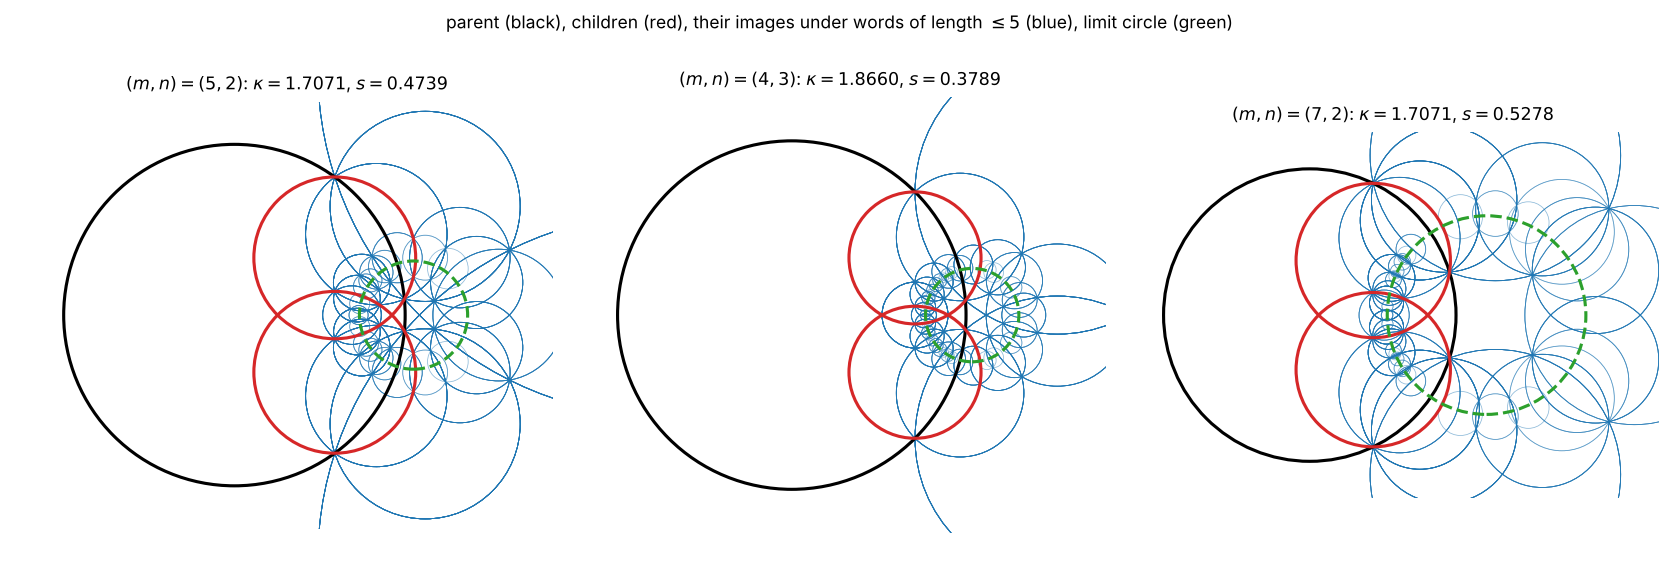
\includegraphics[width=\linewidth]{hopf_reflection.png}
\caption{The parent (black) and children (red) circles in the plane of their centres, their images under reduced words of length at most $5$ (blue) and the common orthogonal circle (green, dashed) for $(m,n)=(5,2),(4,3),(7,2)$.}
\label{fig:reflection}
\end{figure}

\subsection{Planar Limit Circles and Boundaries of the Reflection Family}

\begin{itemize}[leftmargin=*,itemsep=2pt]
\item The Hopf clasp is the $n=2$ member of a one-parameter family of clasps, $\kappa_n=1+\cos(\pi/2n)$, whose invariant is $s_1=\cos(\pi/n)$, and for each $\kappa_n$ and each $m$ with $2/m+1/n<1$ there is one shrink $s_m$ for which the ring and its children generate a reflection group.  The oloid's pair occurs as $n=3$ (and as $\kappa=3/2$, which is not in the family).
\item The limit sets of these groups are round circles, so this construction gives a Fuchsian group in a plane and \emph{no} wild limit set.  Wild limit sets need genuinely three-dimensional configurations, as in the constructions cited by the companion~\ref{hopffibration}.
\item The horned-sphere trees at these parameters are not all embedded at depth 3: the Hopf cases $(5,2),(6,2),(7,2)$ and $(4,3)$ have no extra touching pairs and 39 linked pairs; $(5,3)$ and $(3,4)$ have extra touching pairs.  The tube clearance was not computed.
\item The pseudo-Kleinian field is not one of these groups: its box fold is a reflection in planes, but the clamp and the single inversion in a fixed sphere with the accumulated scale $T$ do not obviously generate a discrete group, and we have not tested whether they do.  Whether inversions in the rings of the tree, in place of a fixed sphere, give a distance field with a Kleinian limit set is an open question.
\end{itemize}



\section{Limitations and open questions}
\label{sec:limits}

\begin{itemize}[leftmargin=*,itemsep=2pt]
\item \emph{Linking is of centre circles.}  We compute linking numbers of completed circles, not of the tube surfaces with their cut.  Where the tubes are disjoint ($t$ below $t_{\max}$) the cores' linking describes the tubes; where they are not, it does not.  Changes of the linking graph with $\psi$ happen when two completed circles cross, possibly inside a removed cut, so they need not correspond to any contact between the physical tubes.  We make no claim that the limit set of a Hopf tree is a wild or tame sphere.
\item \emph{Depth.}  Linking graphs were computed to depth 3 for the scans and depth 4 for selected cases.  Whether the grandchild rule persists at depths 5 and beyond, and why it ends at $\psi=221^\circ$, is open.
\item \emph{Parameters.}  All the Hopf-tree results are for $s=0.4$ and, apart from the mirror symmetry, hang $=+1$.  The dependence on $s$ is only through \cref{eq:hopf_gap} and the clearance $t_{\max}$ and has not been scanned.
\item \emph{Proof status.}  \Cref{lem:smin,prop:prune,prop:hopf,prop:selfsim} are proved above (the first two also tested).  The regimes in $\psi$ and \cref{obs:rule} are empirical.
\item \emph{Clasp scan.}  \Cref{tab:clasp} is for $s=0.4$, depth 3 and one \code{turn}; tube clearance was not computed there, and \cref{obs:hopf_is_horned} is a numerical equality at $s=0.4$ only.
\item \emph{Reflection groups.}  \Cref{sec:kleinian} verifies the Coxeter relations numerically and relies on the classical polygon theorem for discreteness and for the limit circle; the pseudo-Kleinian is only compared by name.
\item \emph{Distance estimates.}  The Hopfbrot and Riemann-sphere estimates are heuristics ported from ray, not proven bounds, and hybrids mix estimates that disagree.  Hybrid renderings should be read as explorations.
\end{itemize}


\section{Conclusion}

Representing recursive fractals and fibre networks within a unified distance-field framework makes it possible to probe their global topology directly rather than relying solely on visual cross-sections. Starting from an exact, order-independent distance estimator for Alexander's horned sphere, we proved that pruned breadth-first evaluation equals the full tree minimum (Lemma~1 and Proposition~2), while its underlying skeleton of circles admits a direct topological comparison with the Hopf fibration.

Replacing the hand-placed clasp of the horned sphere with stereographically projected Hopf pairs collapses the clasp geometry onto a single placement parameter $\psi$ along the Clifford torus. While most placements preserve the sibling-only linking graph of the classical horned sphere, the thick-tube window $202^\circ \le \psi \le 221^\circ$ exhibits a repeatable, generation-invariant grandchild linking rule ($Lk = -1$ and $+1$) with non-overlapping tubes. Analyzing the clasp via its Lorentz-model Gram matrix yields the closed-form M\"obius invariant $s_1(\kappa) = |1 - 2(\kappa - 1)^2|$, unifying the exact Hopf clasp ($\kappa = 1 + 1/\sqrt{2}$, where the Hopf tree at $\psi = 180^\circ$ coincides with the horned sphere) and the oloid pair ($\kappa = 3/2$) as members of a discrete family $\kappa_n = 1 + \cos(\pi/2n)$ whose equatorial sphere inversions generate planar Coxeter reflection groups.

Together with the fibration equivariance of the Hopfbrot power map, these results show how composable distance fields bridge ray-marched fractal geometry and low-dimensional topology. Proving the boundaries of the empirical grandchild linking regime analytically, and determining whether three-dimensional tree-based sphere inversions generate wild Kleinian limit sets, remain open directions for future work.

\appendix
\footnotesize

\section{Reproducibility}
\label{sec:repro}

The package is in \code{fractalkit/} of the repository~\url{https://github.com/brentharts/ray}; figures are produced by the scripts in \code{examples/}.  The 69 tests in \code{tests/} cover the operators, hybrids, the symbolic checks, comparisons with literal scalar transcriptions of the Rust kernels by Brandon Hoult (2026), the equivalence of the pruned and brute-force horned search, and the linking results.

\subsection{Hopf-Fibration}
\label{hopffibration}
Scripts and notes on the Hopf fibration, the oloid and Antoine's necklace
\newline
\url{https://github.com/brentharts/HopfFibration}

\section{Numerical notes}
\label{sec:numerics}

Box counting: We estimate the box-counting dimension~\cite{falconer2014} by occupancy of a grid on the sign of the field and a log--log regression.  The estimate is exact only if the grid base matches the fractal's scaling: for the Menger sponge with base 3 we measure $2.727$ against $\log20/\log3=2.727$, and for the Sierpinski tetrahedron with base 2 we measure $2.000$ against $\log4/\log2=2$.  With a mismatched base, or a threshold that thickens the occupied set, estimates are biased high.

The bulb estimate: The scalar estimate $n r^{n-1}$ is a lower bound on the spectral norm of the Jacobian of the Mandelbulb power map (symbolically computed with sympy and evaluated at random points): over 20\,000 points with $0.3\le r\le1.2$ at $n=8$ the ratio is at least $1.000$ with median $1.000$ and maximum $7.99$, near the poles.  The estimate is therefore not a distance bound and the bulb must be marched with a step factor below 1; this is the usual practice and consistent with the discussions in~\cite{hvidtfeldt_de,quilez_distance}.



\bibliographystyle{plainnat}
\bibliography{references}

\end{document}
